\subsection{Kinematics vs SUSY Masses} \label{sec::App::kineMap}
The trend of the kinematical variables over the mass grids are shown in Figure \ref{fig::SRdefinition::kineMap_QQC1QQC1_x12}-\ref{fig::SRdefinition::kineMap_TTN1TTN1}. The color scale (z-axis) indicates the mean of the distribution of the variable that the the signal events in the mass point result in. The examples of three \textbf{QQC1QQC1} grids ($\xhalf$, $\varx$, $\DMth$) and one \textbf{TTN1TTN1} grid are shown. 
While the variables related to transverse momenta of outgoing particles such as $\meffInc$, $\lepPt$ and $\met$ simply scale with the mass splitting, the other variables (e.g. aplanarity, $\metOverMeff$ etc.) typically vary depending on the relative mass spilitting, the cuts in which are therefore helpful for segmenting the signal region towers.
These are used in deciding the initial cuts for the signal regions optimization. \\


%\clearpage
    
\begin{figure}[h]
  \centering
%    \subfigure[]{\includegraphics[width=0.45\textwidth]{figures/SRdefinition/kineMap/GG_symQQC1_x12_nJet30.pdf}}
    \subfigure[]{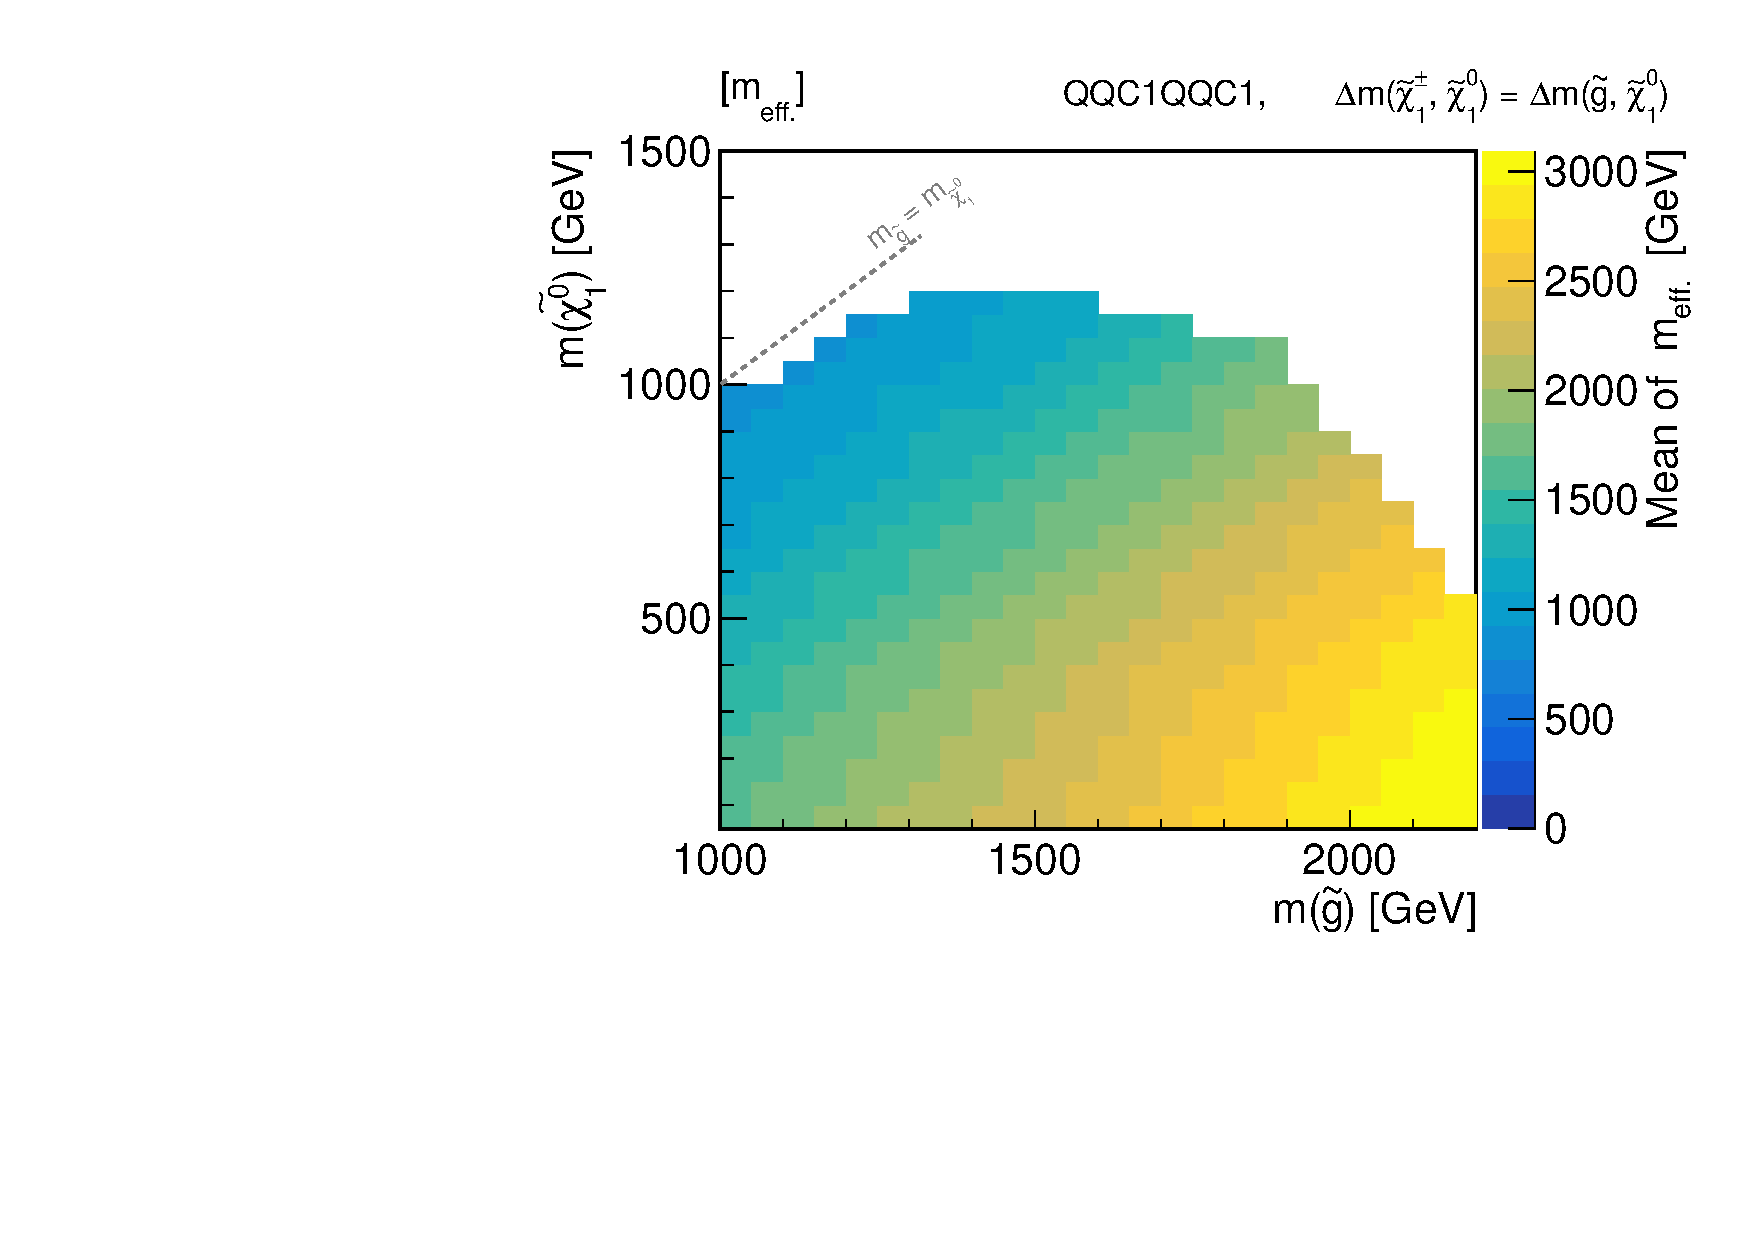
\includegraphics[width=0.45\textwidth]{figures/SRdefinition/kineMap/GG_symQQC1_x12_meff.pdf}}
    \subfigure[]{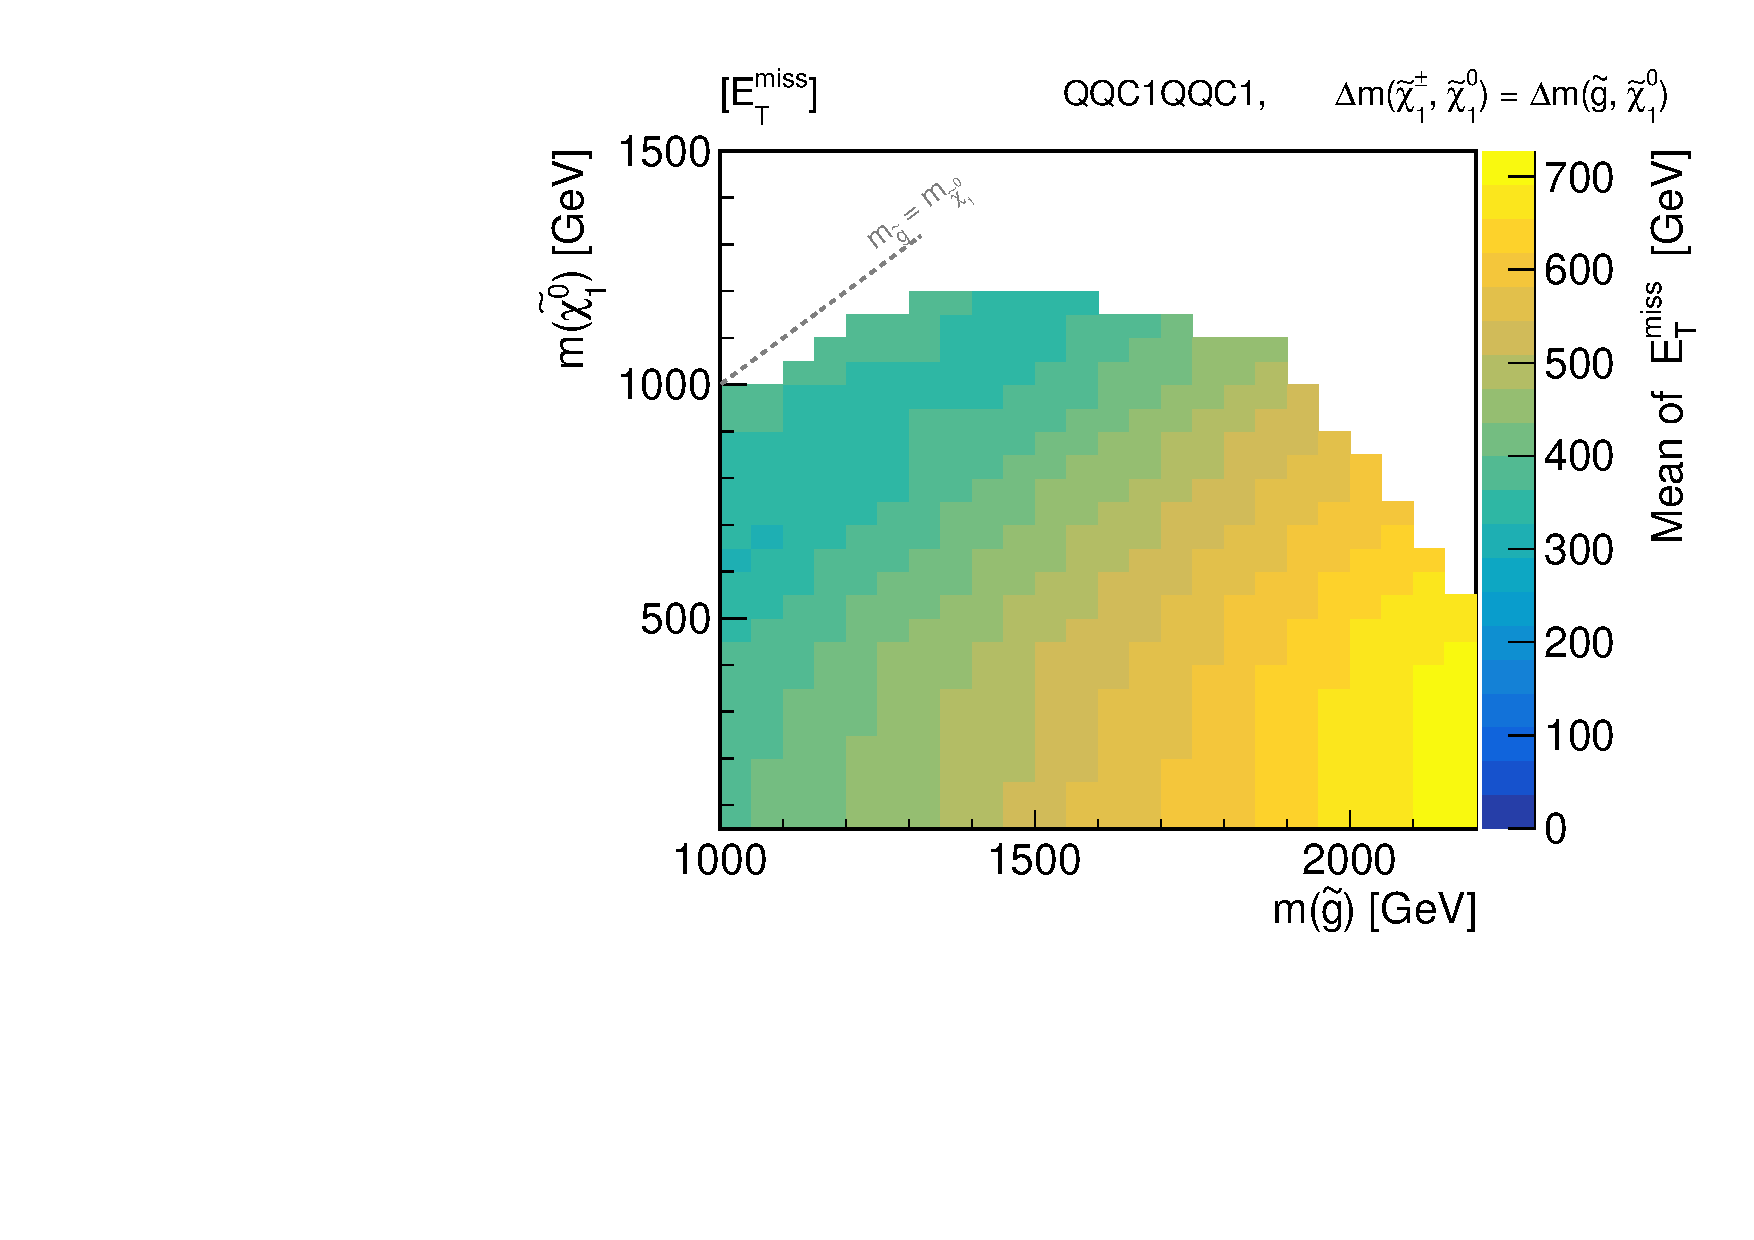
\includegraphics[width=0.45\textwidth]{figures/SRdefinition/kineMap/GG_symQQC1_x12_met.pdf}}
    \subfigure[]{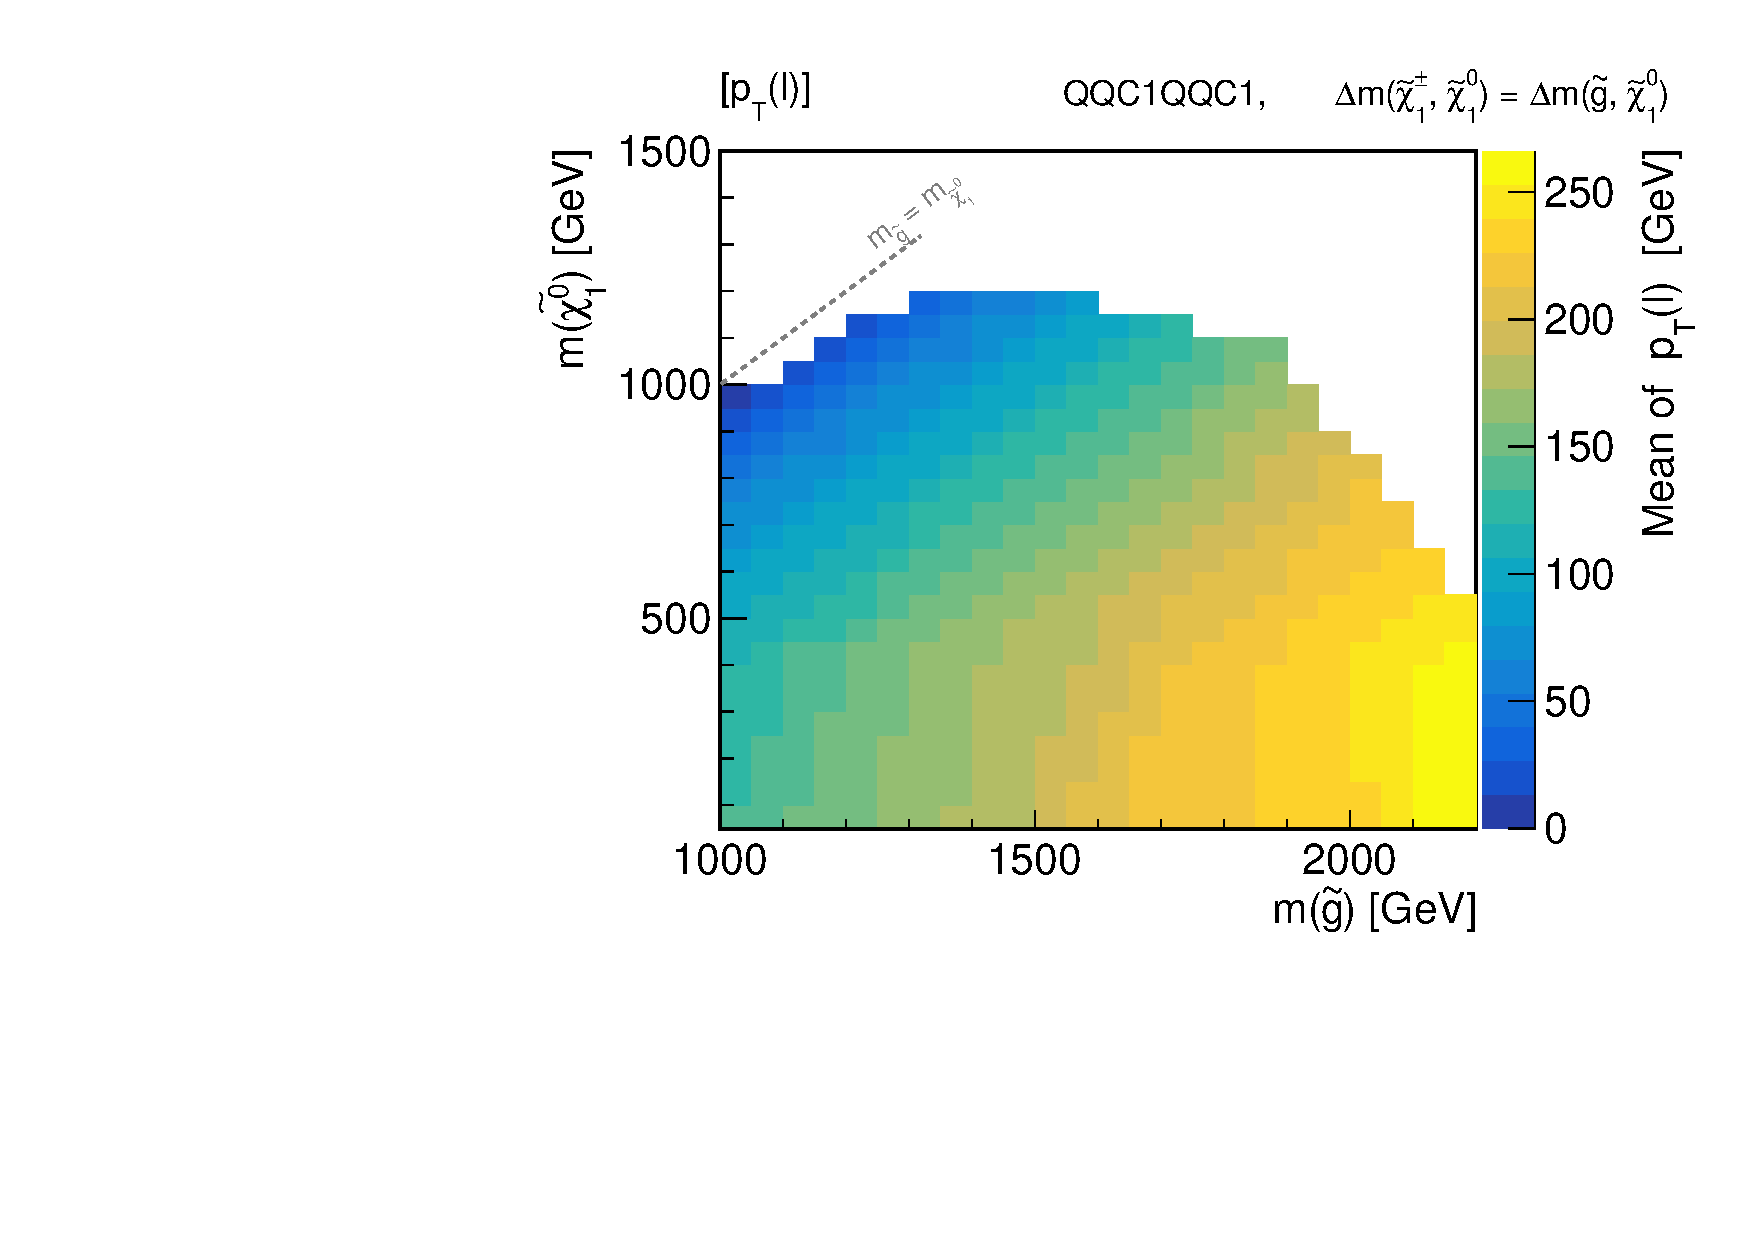
\includegraphics[width=0.45\textwidth]{figures/SRdefinition/kineMap/GG_symQQC1_x12_lep1Pt.pdf}}
    \subfigure[]{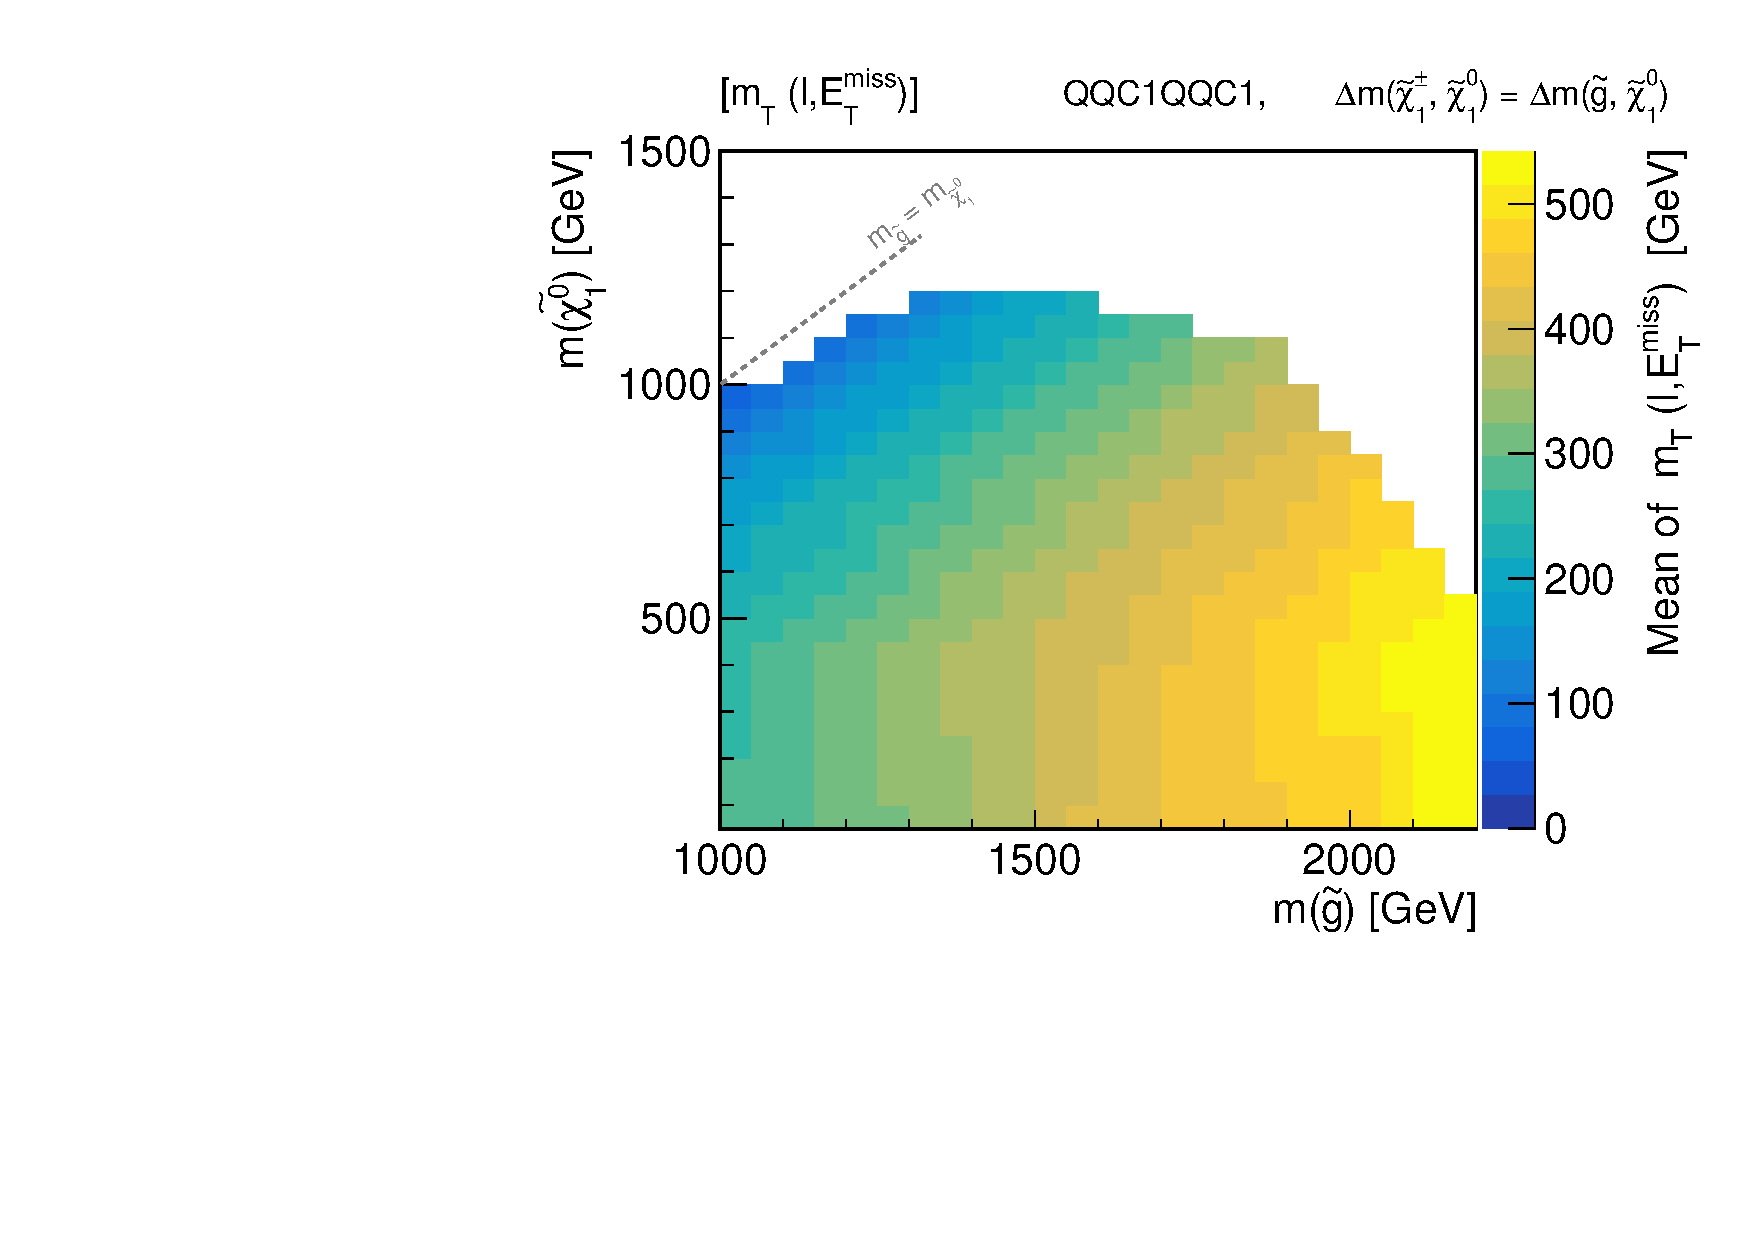
\includegraphics[width=0.45\textwidth]{figures/SRdefinition/kineMap/GG_symQQC1_x12_mt.pdf}}
    \subfigure[]{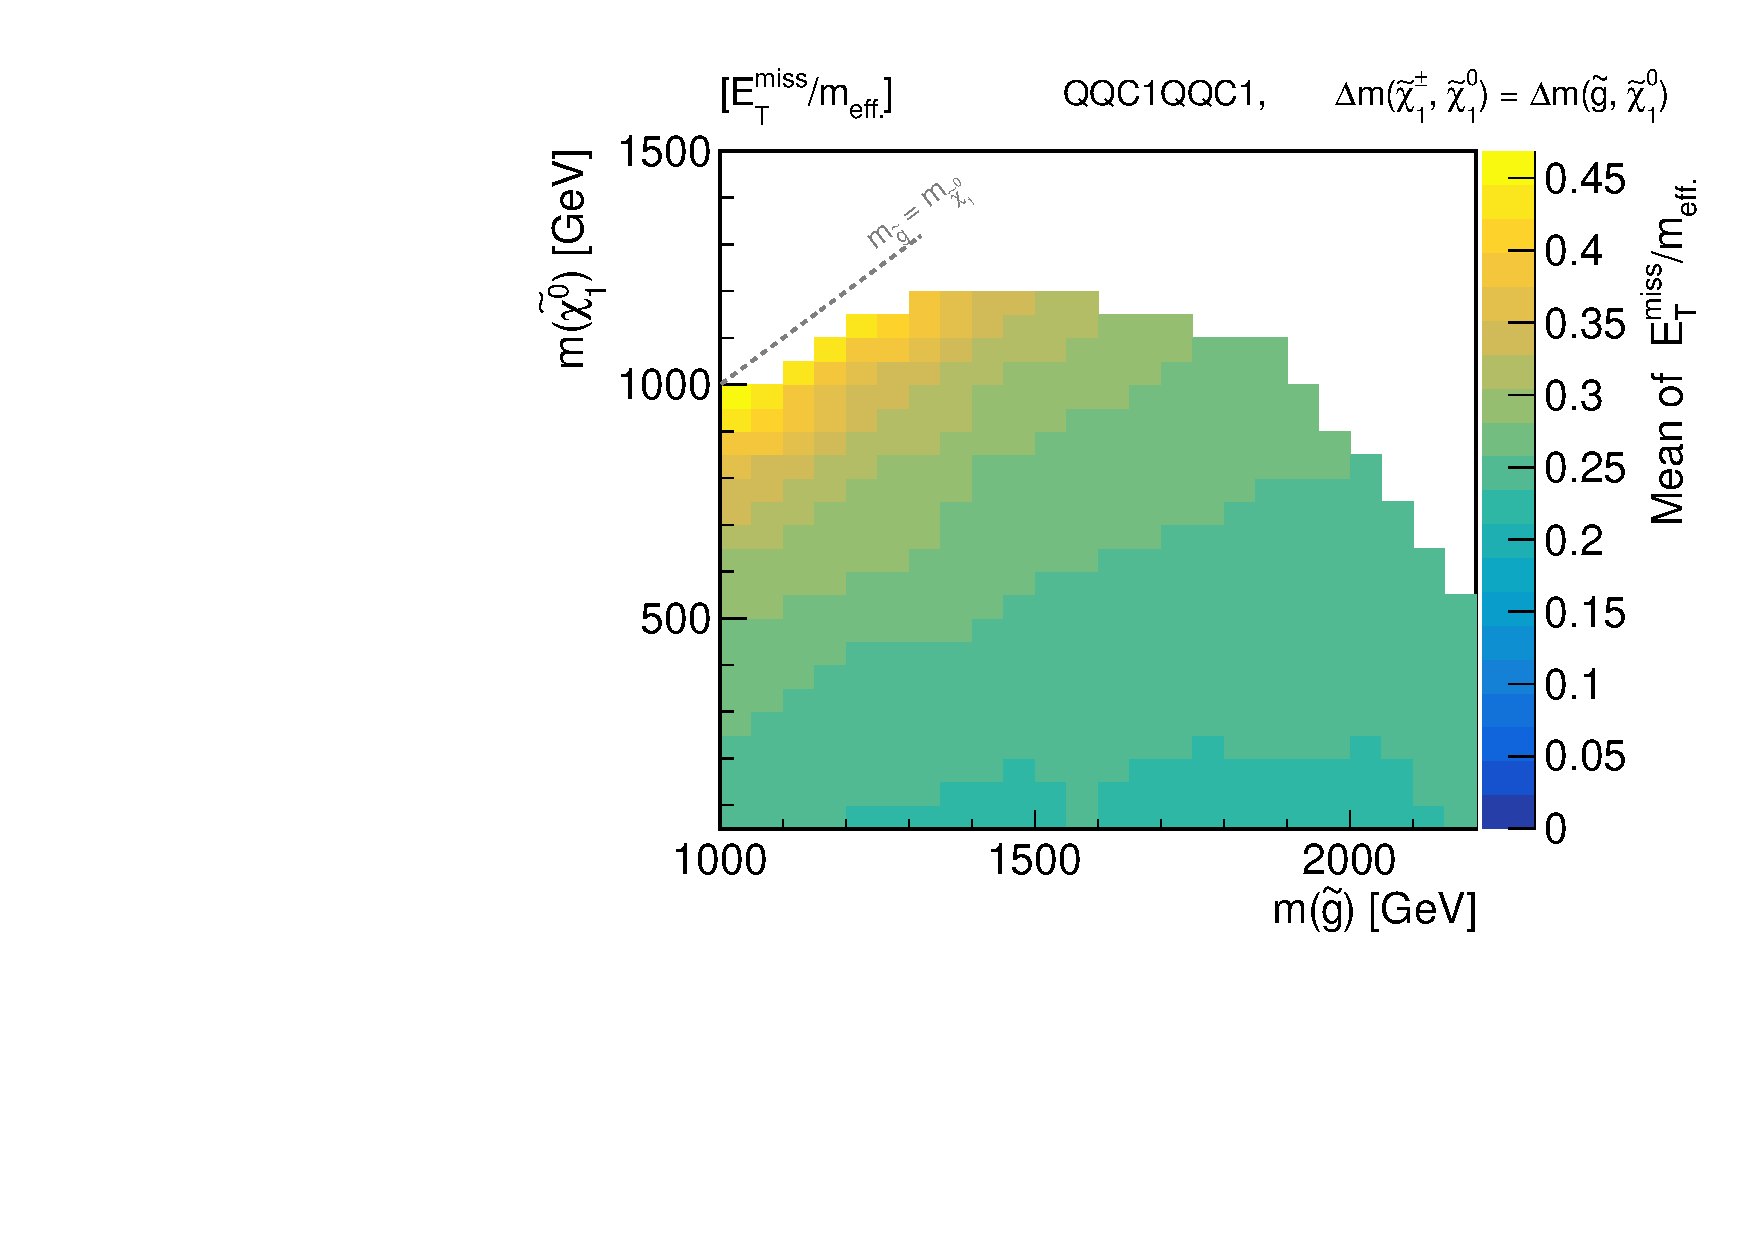
\includegraphics[width=0.45\textwidth]{figures/SRdefinition/kineMap/GG_symQQC1_x12_metOverMeff.pdf}}
    \subfigure[]{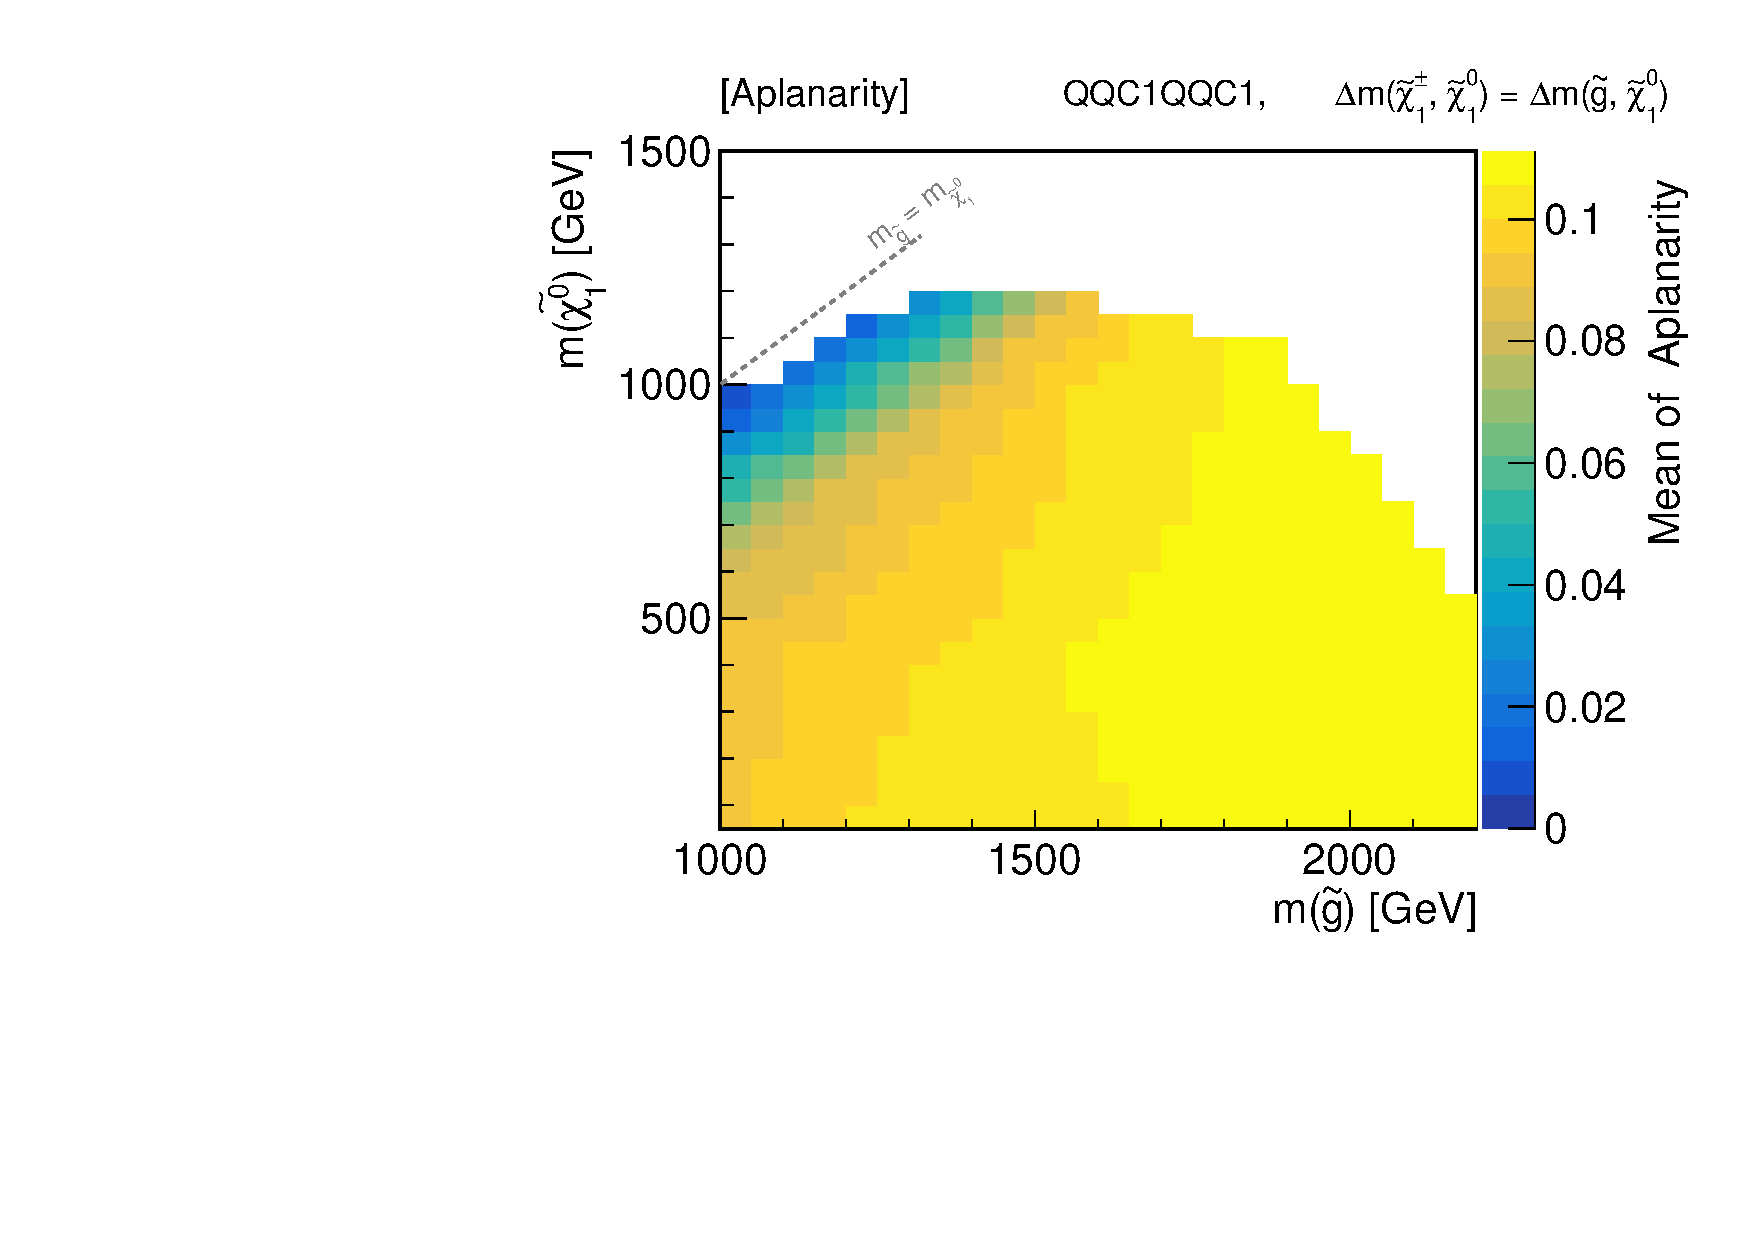
\includegraphics[width=0.45\textwidth]{figures/SRdefinition/kineMap/GG_symQQC1_x12_LepAplanarity.pdf}}
    \caption{ Mean of (a) $\meffInc$ (b) $\met$ (c) $\lepPt$ (d) $\mt$ (e) $\metOverMeff$ (f) aplanarity, for the QQC1QQC1 \xhalf grid, after the pre-selection. 
      \label{fig::SRdefinition::kineMap_QQC1QQC1_x12} 
    }
\end{figure}
 

\begin{figure}[h]
  \centering
%    \subfigure[]{\includegraphics[width=0.45\textwidth]{figures/SRdefinition/kineMap/GG_symQQC1_varx_nJet30.pdf}}
    \subfigure[]{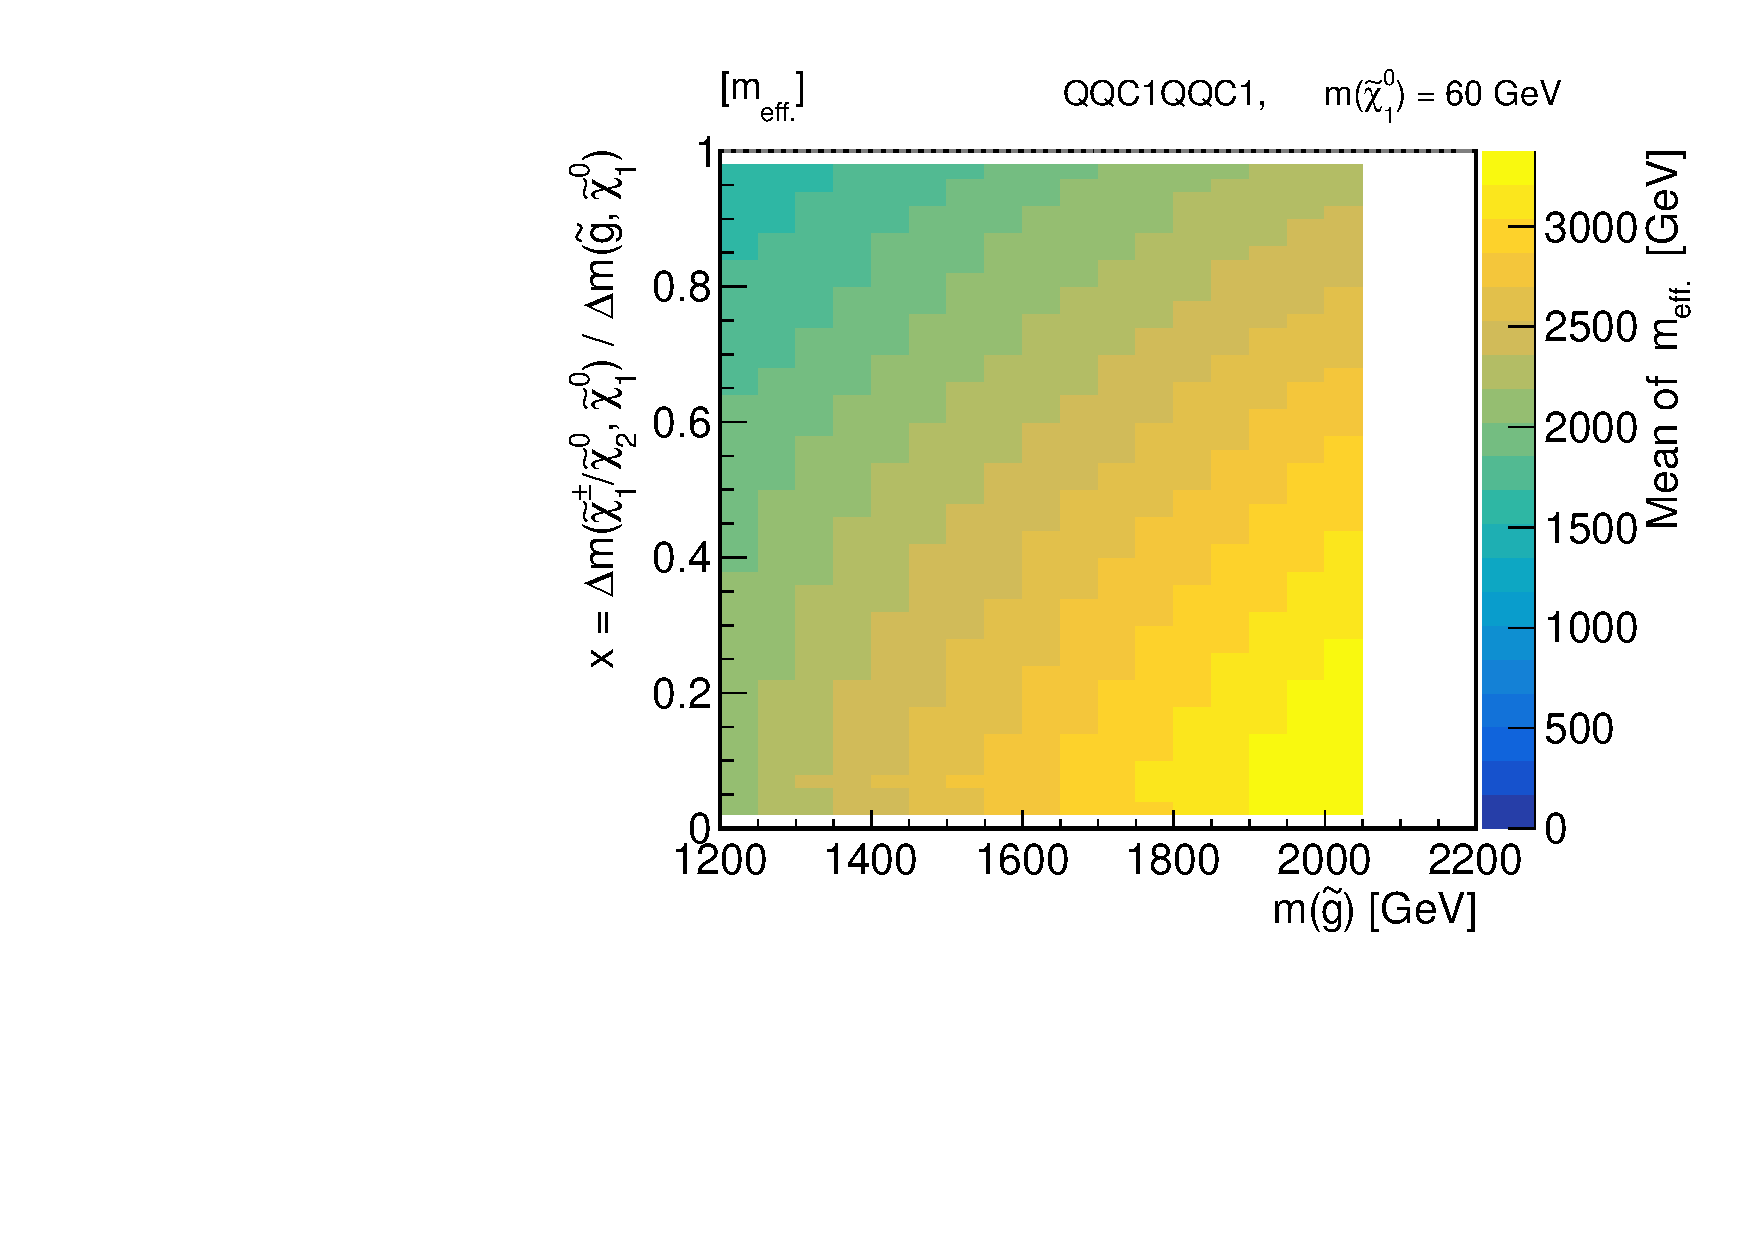
\includegraphics[width=0.45\textwidth]{figures/SRdefinition/kineMap/GG_symQQC1_varx_meff.pdf}}
    \subfigure[]{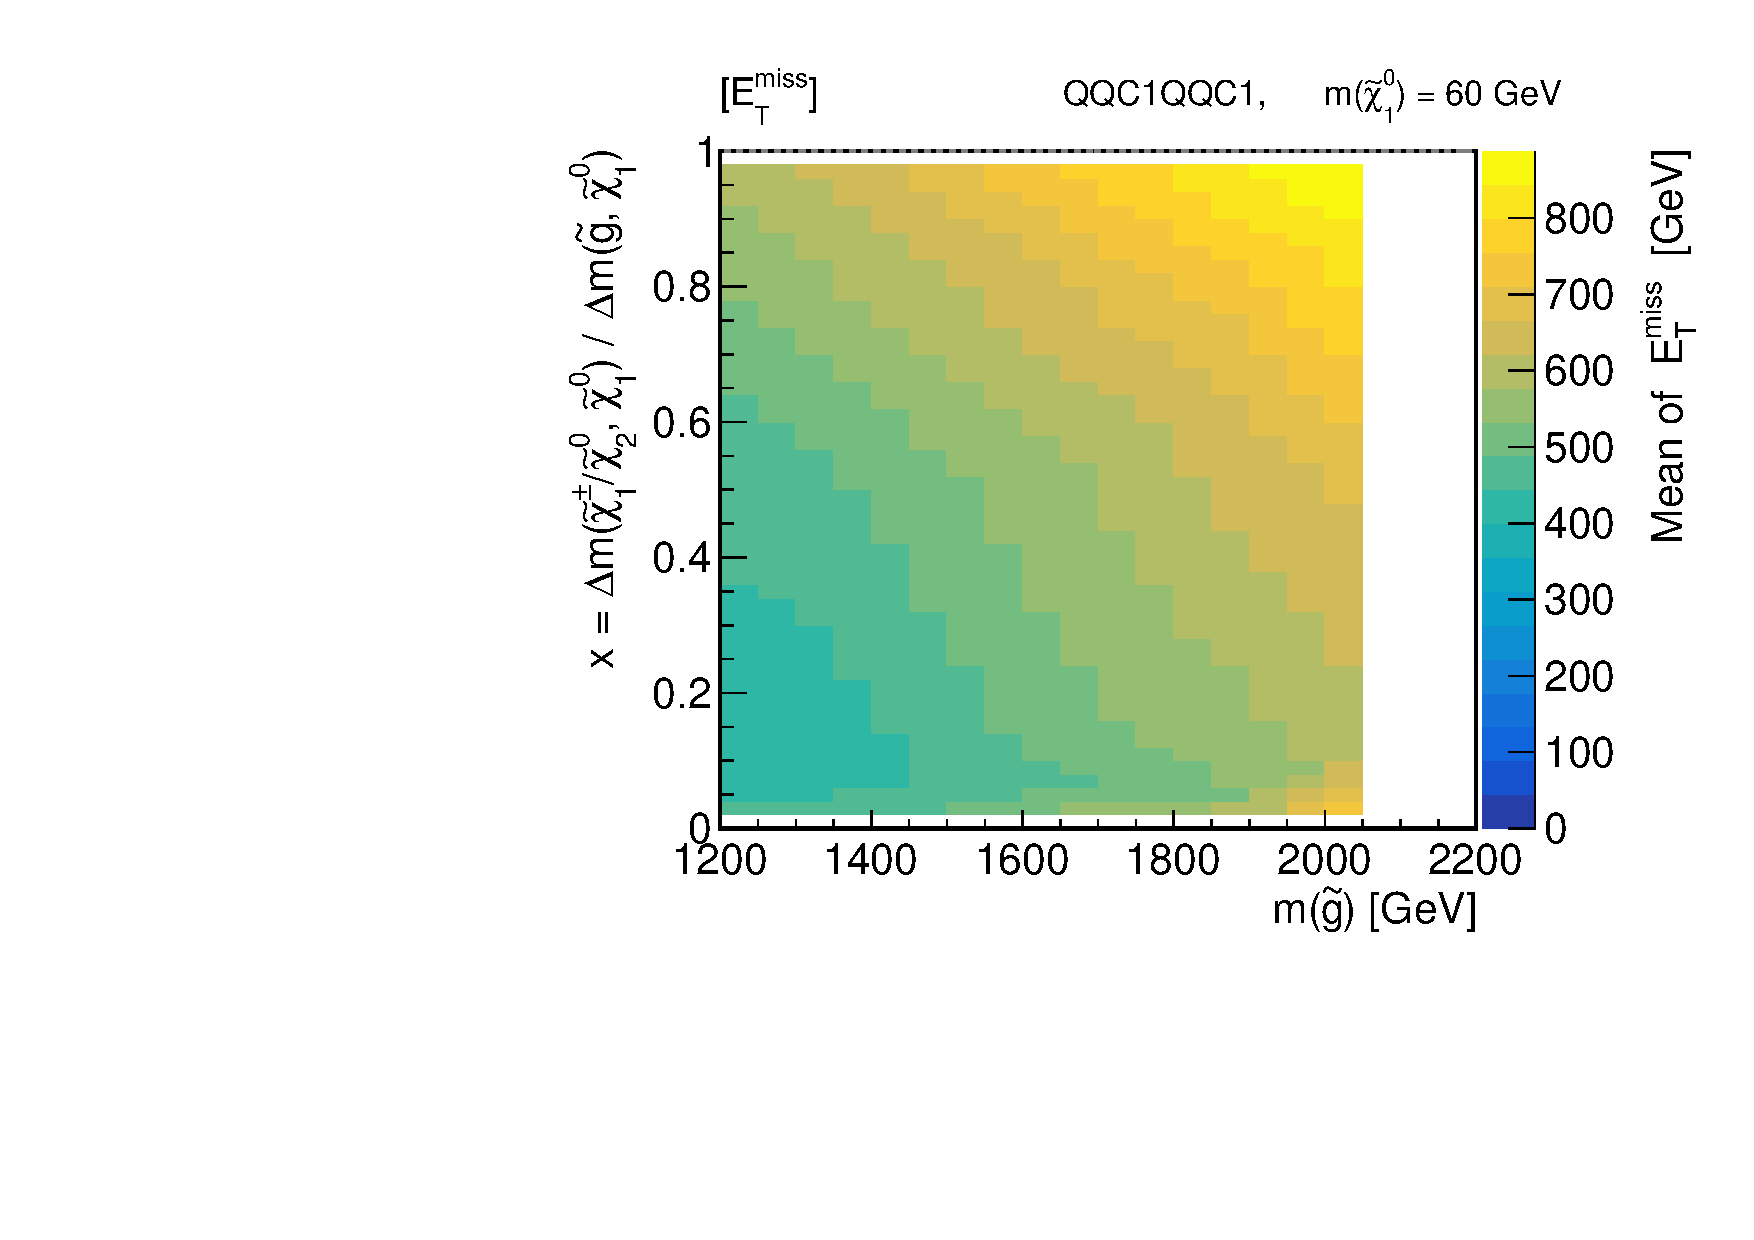
\includegraphics[width=0.45\textwidth]{figures/SRdefinition/kineMap/GG_symQQC1_varx_met.pdf}}
    \subfigure[]{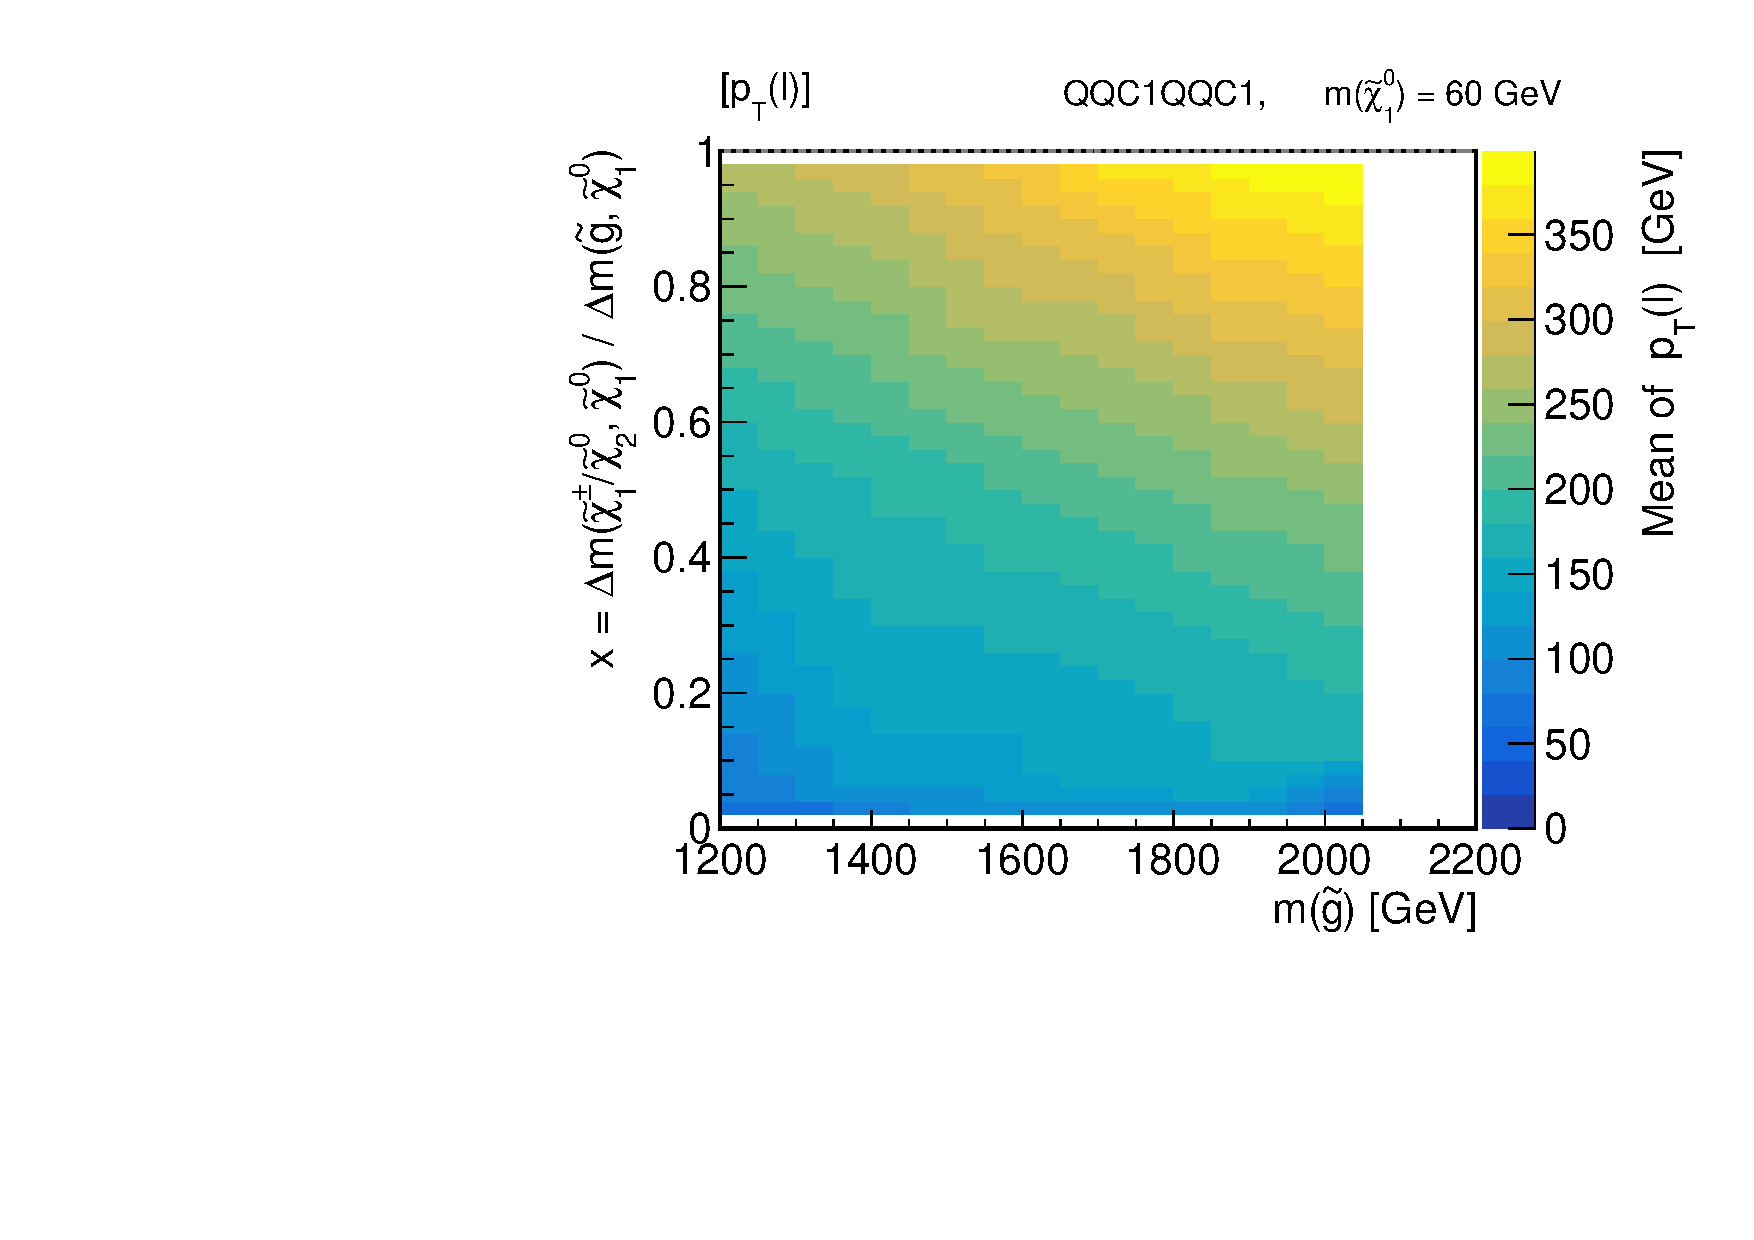
\includegraphics[width=0.45\textwidth]{figures/SRdefinition/kineMap/GG_symQQC1_varx_lep1Pt.pdf}}
    \subfigure[]{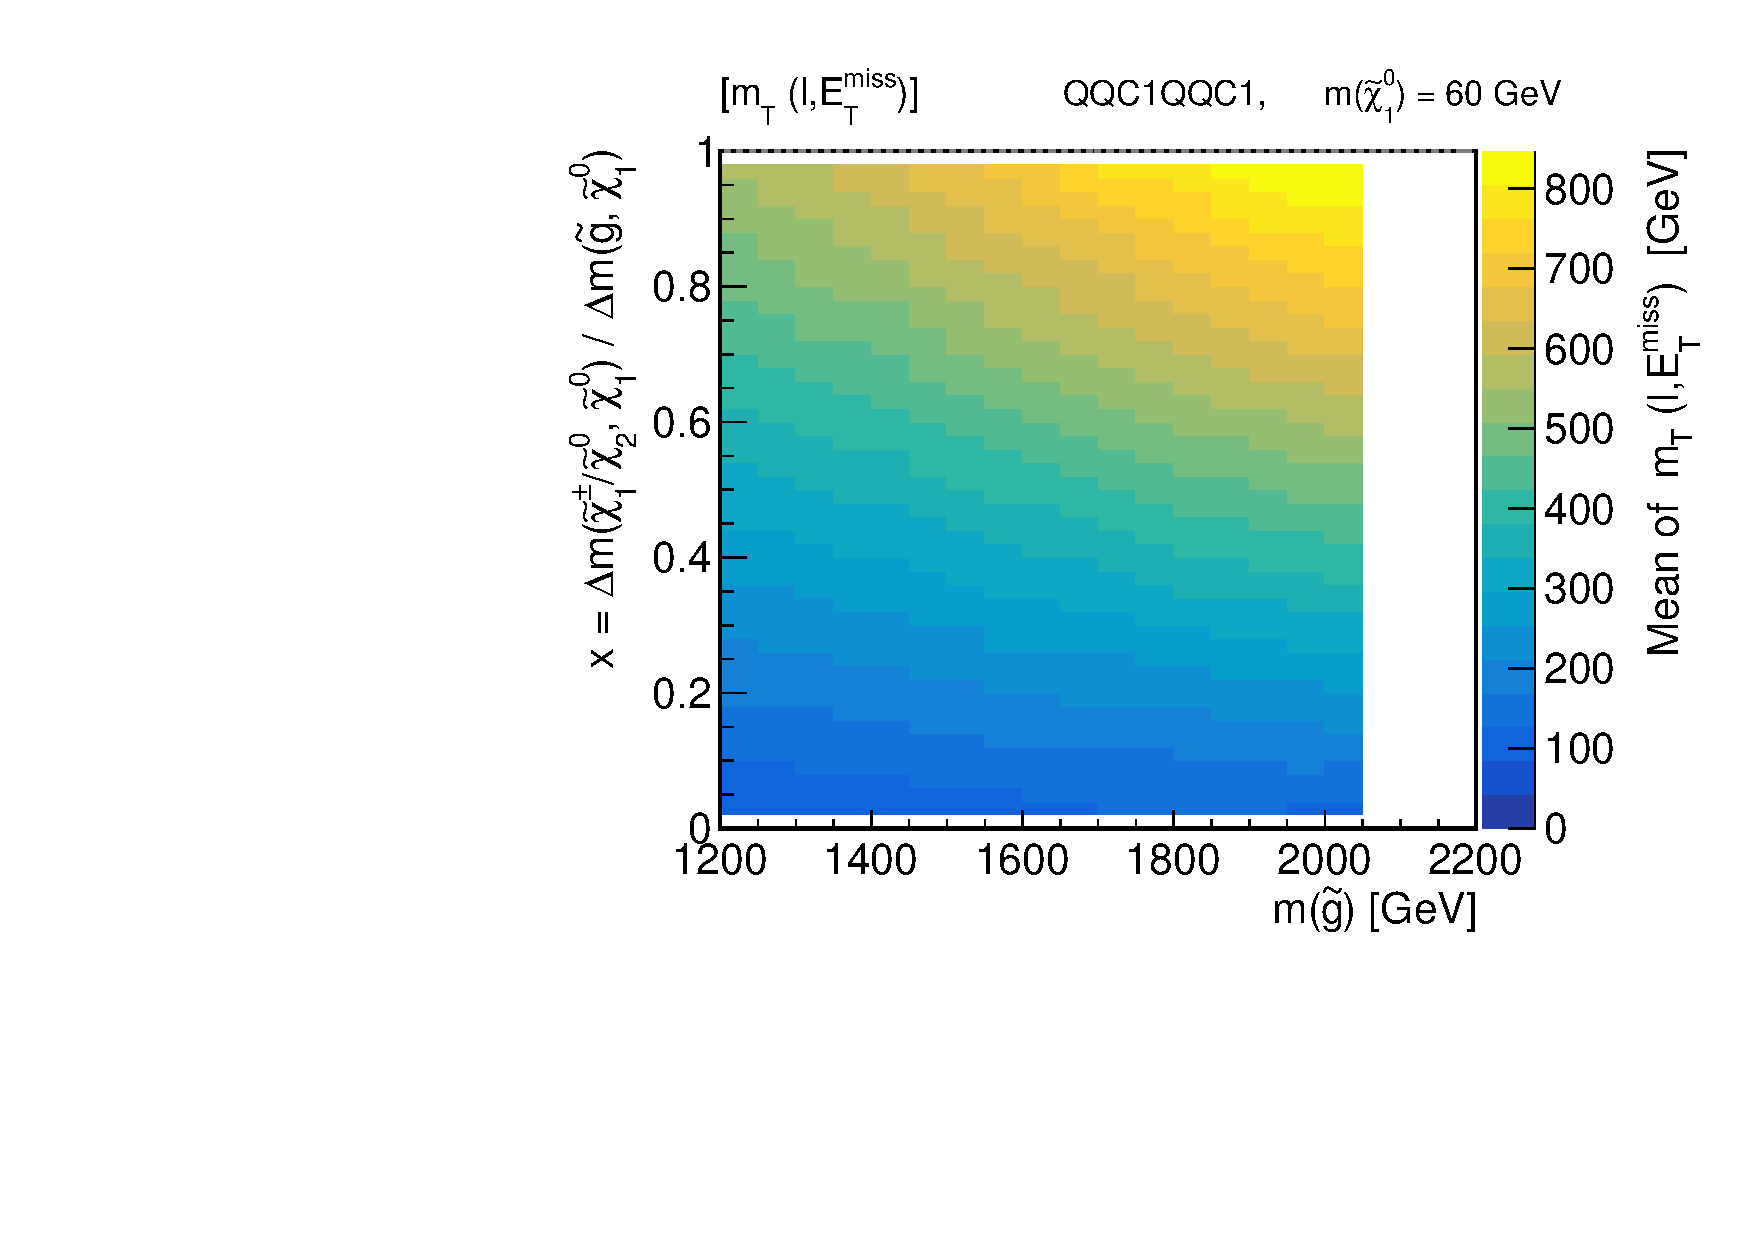
\includegraphics[width=0.45\textwidth]{figures/SRdefinition/kineMap/GG_symQQC1_varx_mt.pdf}}
    \subfigure[]{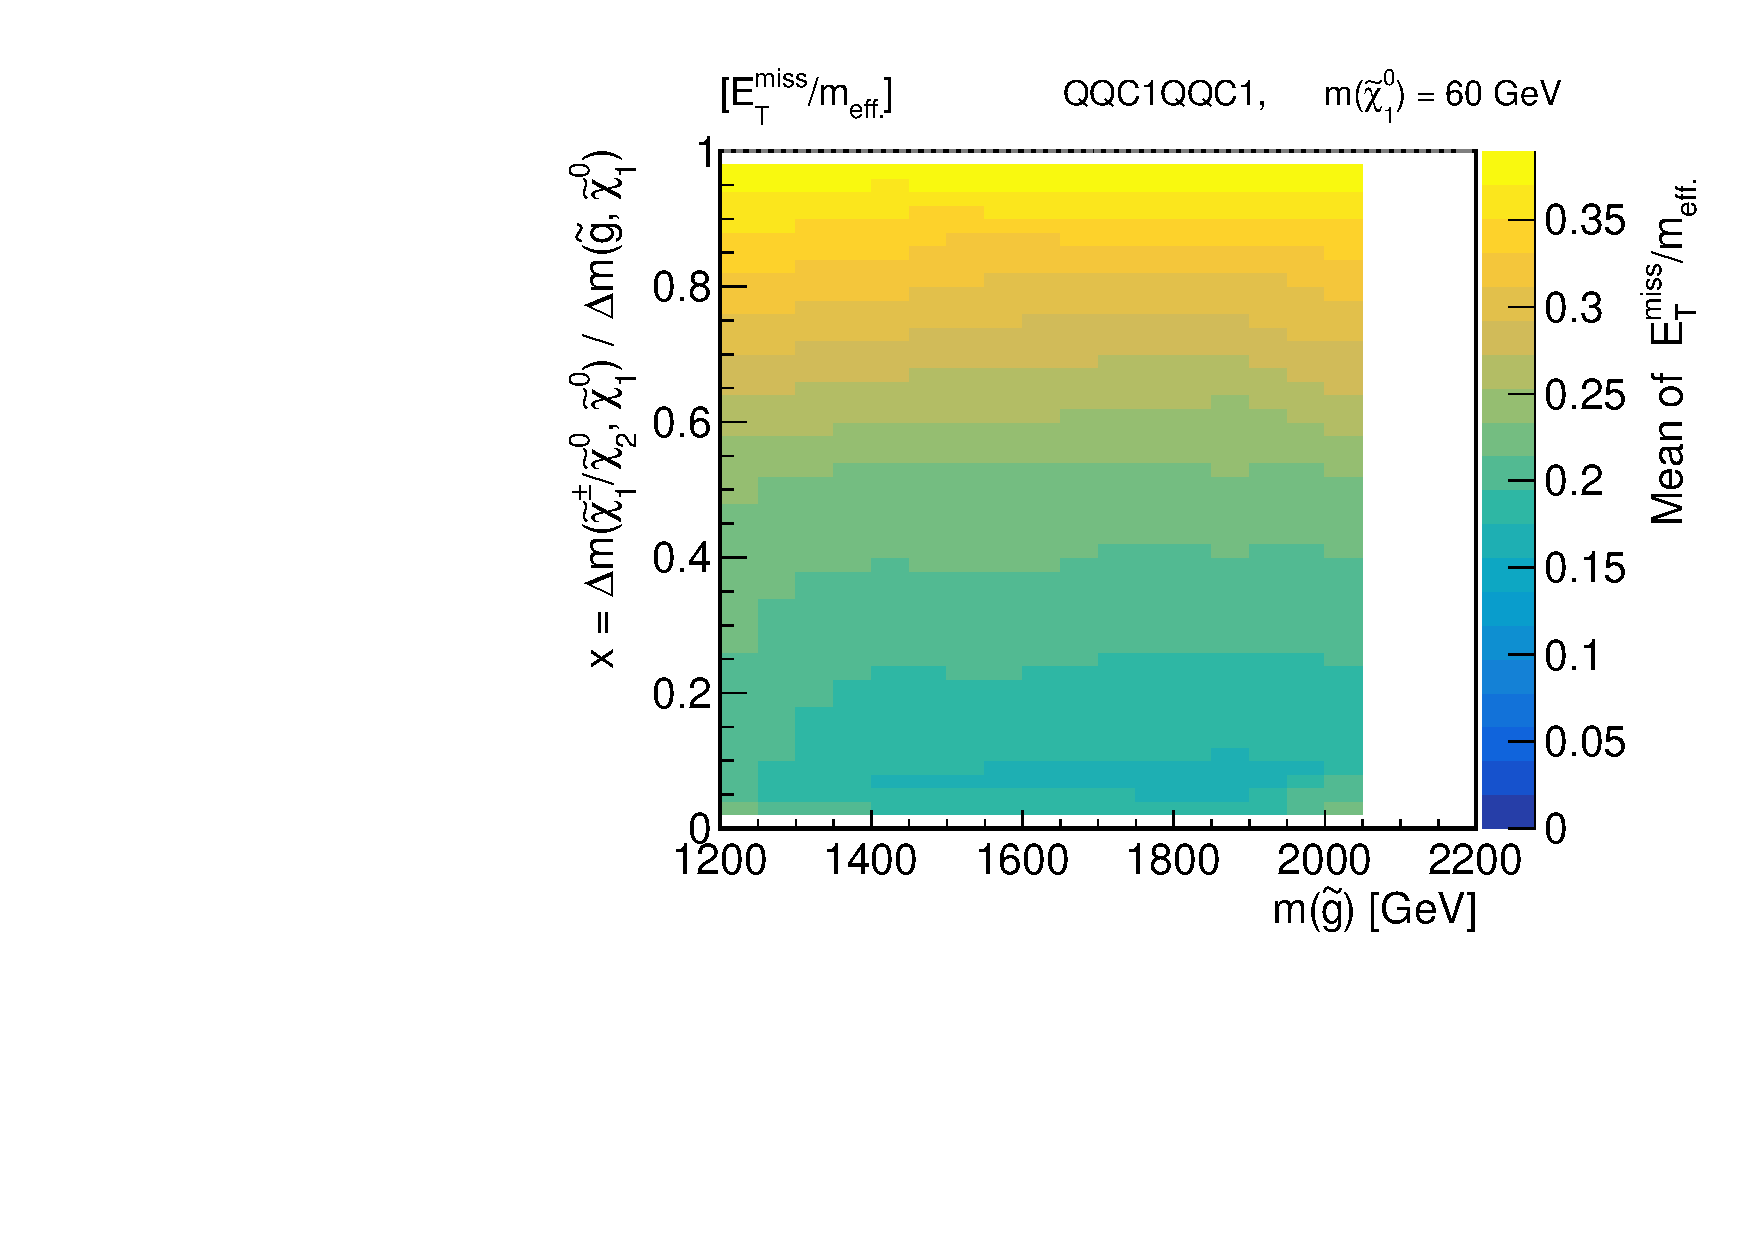
\includegraphics[width=0.45\textwidth]{figures/SRdefinition/kineMap/GG_symQQC1_varx_metOverMeff.pdf}}
    \subfigure[]{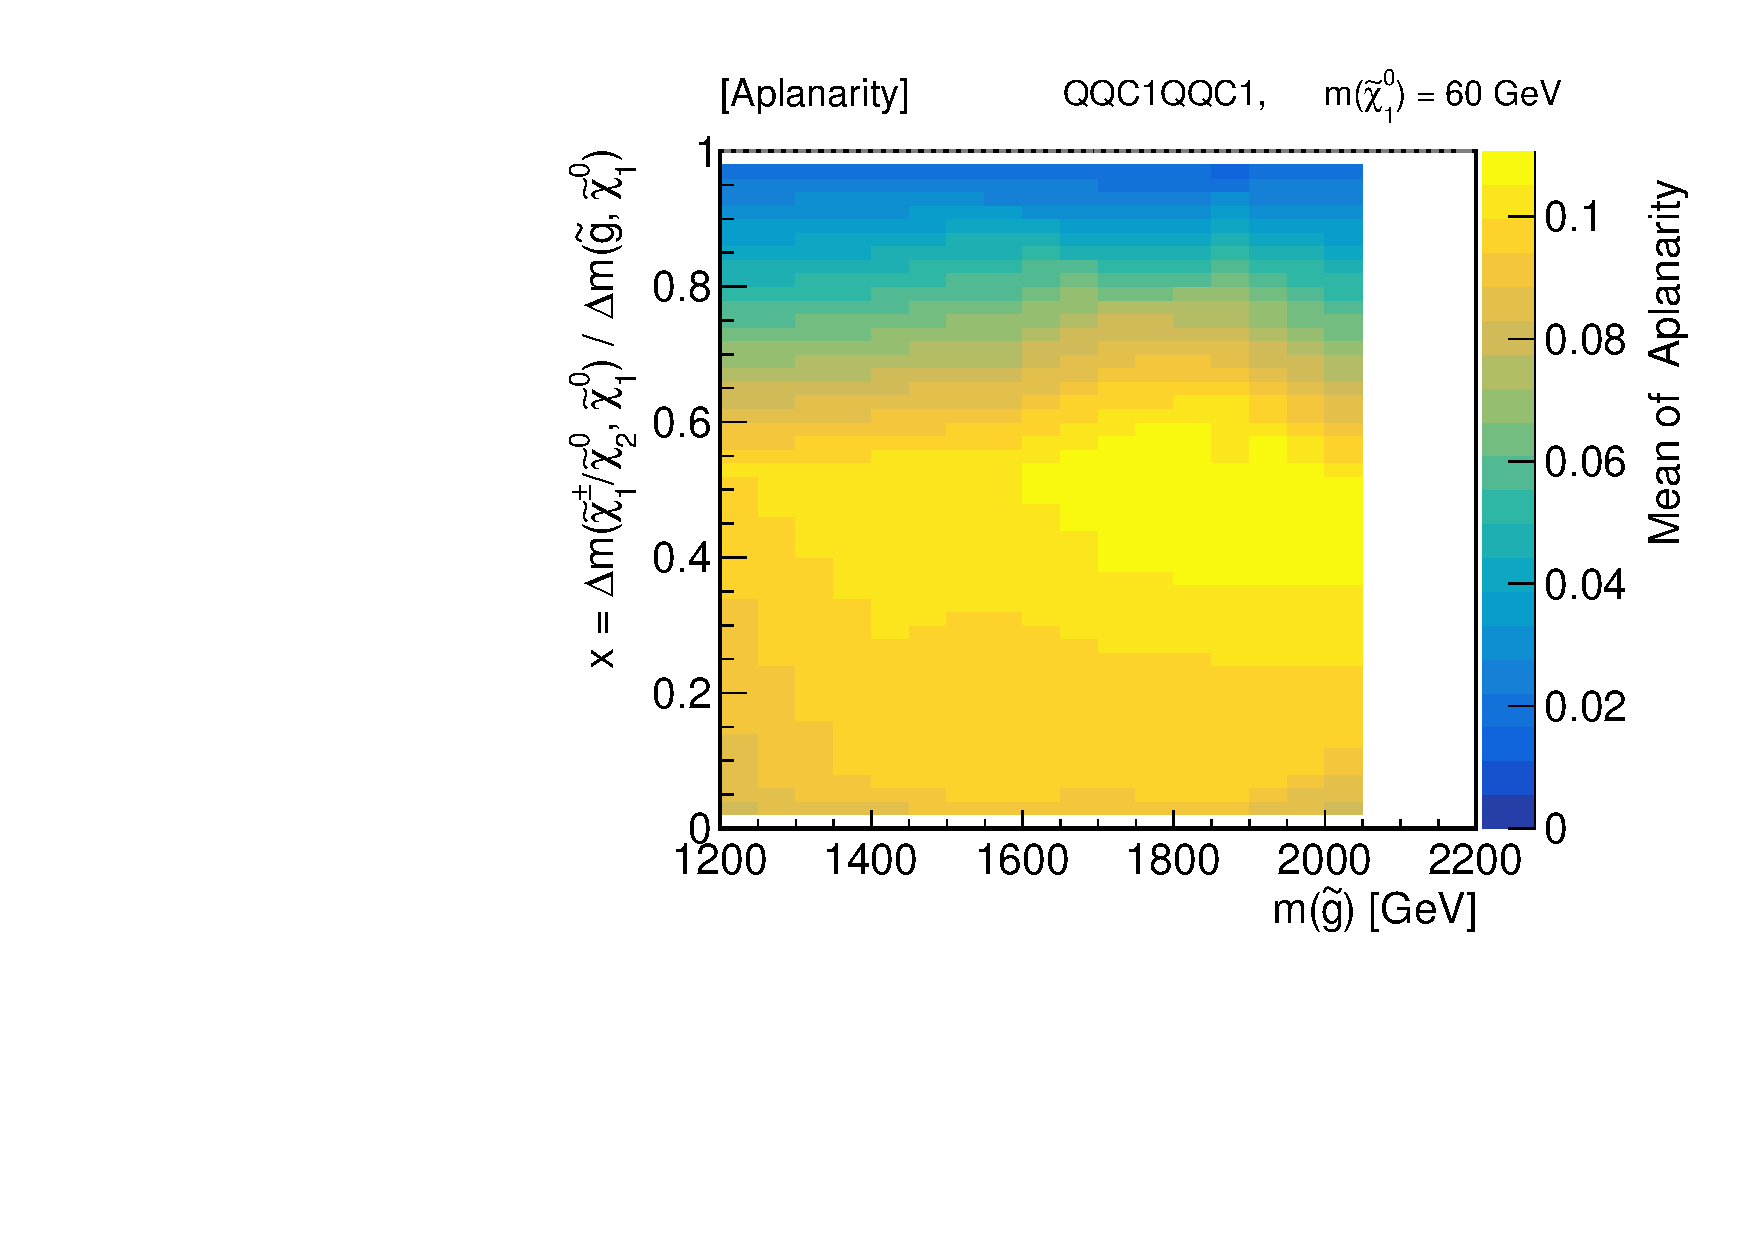
\includegraphics[width=0.45\textwidth]{figures/SRdefinition/kineMap/GG_symQQC1_varx_LepAplanarity.pdf}}
    \caption{ Mean of (a) $\meffInc$ (b) $\met$ (c) $\lepPt$ (d) $\mt$ (e) $\metOverMeff$  (f) aplanarity, for the QQC1QQC1 \varx grid, after the pre-selection. 
      \label{fig::SRdefinition::kineMap_QQC1QQC1_varx} 
    }
\end{figure}

 
%\begin{figure}[h]
%  \centering
%    \subfigure[]{\includegraphics[width=0.45\textwidth]{figures/SRdefinition/kineMap/GG_symQQC1_dM20_nJet30.pdf}}
%    \subfigure[]{\includegraphics[width=0.45\textwidth]{figures/SRdefinition/kineMap/GG_symQQC1_dM20_meff.pdf}}
%    \subfigure[]{\includegraphics[width=0.45\textwidth]{figures/SRdefinition/kineMap/GG_symQQC1_dM20_met.pdf}}
%    \subfigure[]{\includegraphics[width=0.45\textwidth]{figures/SRdefinition/kineMap/GG_symQQC1_dM20_lep1Pt.pdf}}
%    \subfigure[]{\includegraphics[width=0.45\textwidth]{figures/SRdefinition/kineMap/GG_symQQC1_dM20_mt.pdf}}
%    \subfigure[]{\includegraphics[width=0.45\textwidth]{figures/SRdefinition/kineMap/GG_symQQC1_dM20_LepAplanarity.pdf}}
%    \caption{ Mean of (a) jet-multiplicity ($p_T>30\gev$) (b) $\meffInc$ (c) $\met$ (d) $\lepPt$ (e) $\mt$ (f) aplanarity, for the QQC1QQC1 $\Delta M = 20\gev$ grid, after the pre-selection. }
%\end{figure}
 
\begin{figure}[h]
  \centering
%    \subfigure[]{\includegraphics[width=0.45\textwidth]{figures/SRdefinition/kineMap/GG_symQQC1_dM30_nJet30.pdf}}
    \subfigure[]{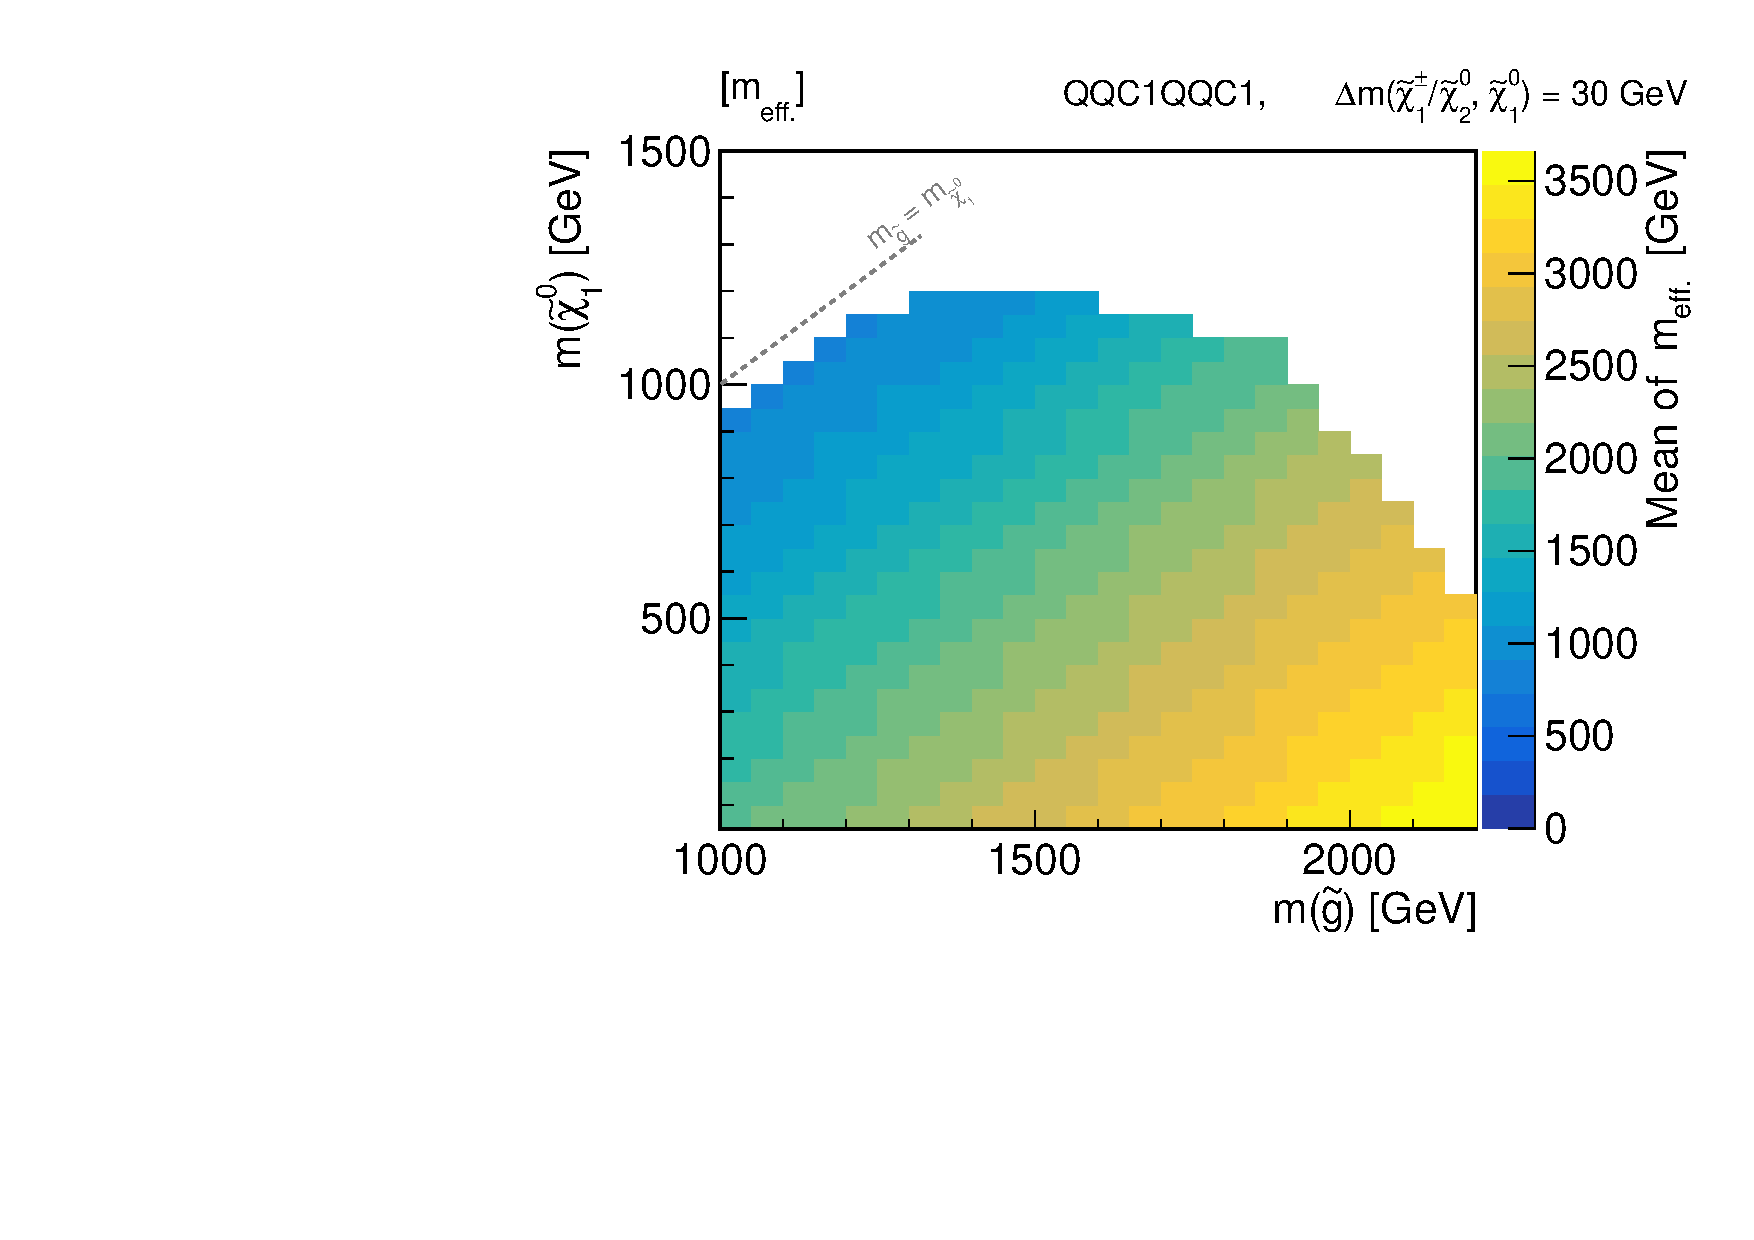
\includegraphics[width=0.45\textwidth]{figures/SRdefinition/kineMap/GG_symQQC1_dM30_meff.pdf}}
    \subfigure[]{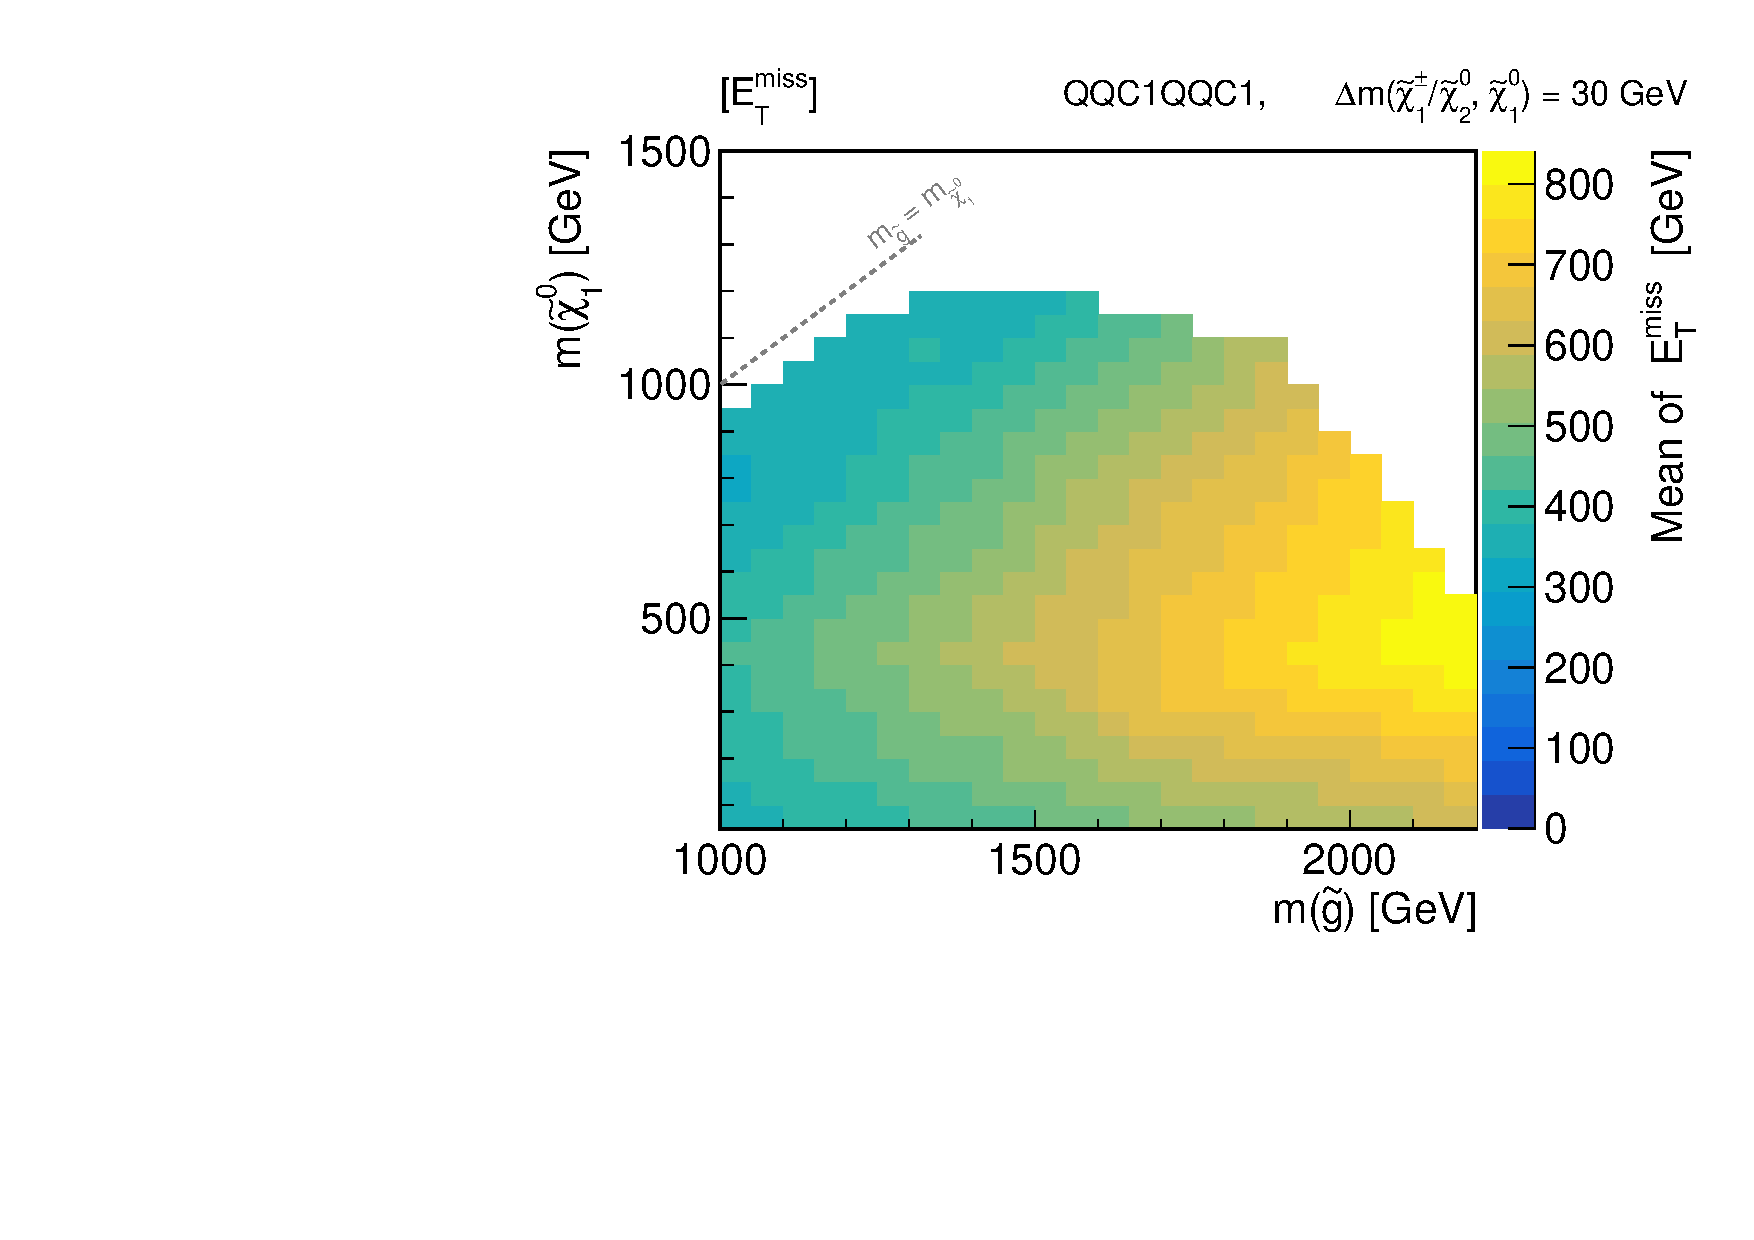
\includegraphics[width=0.45\textwidth]{figures/SRdefinition/kineMap/GG_symQQC1_dM30_met.pdf}}
    \subfigure[]{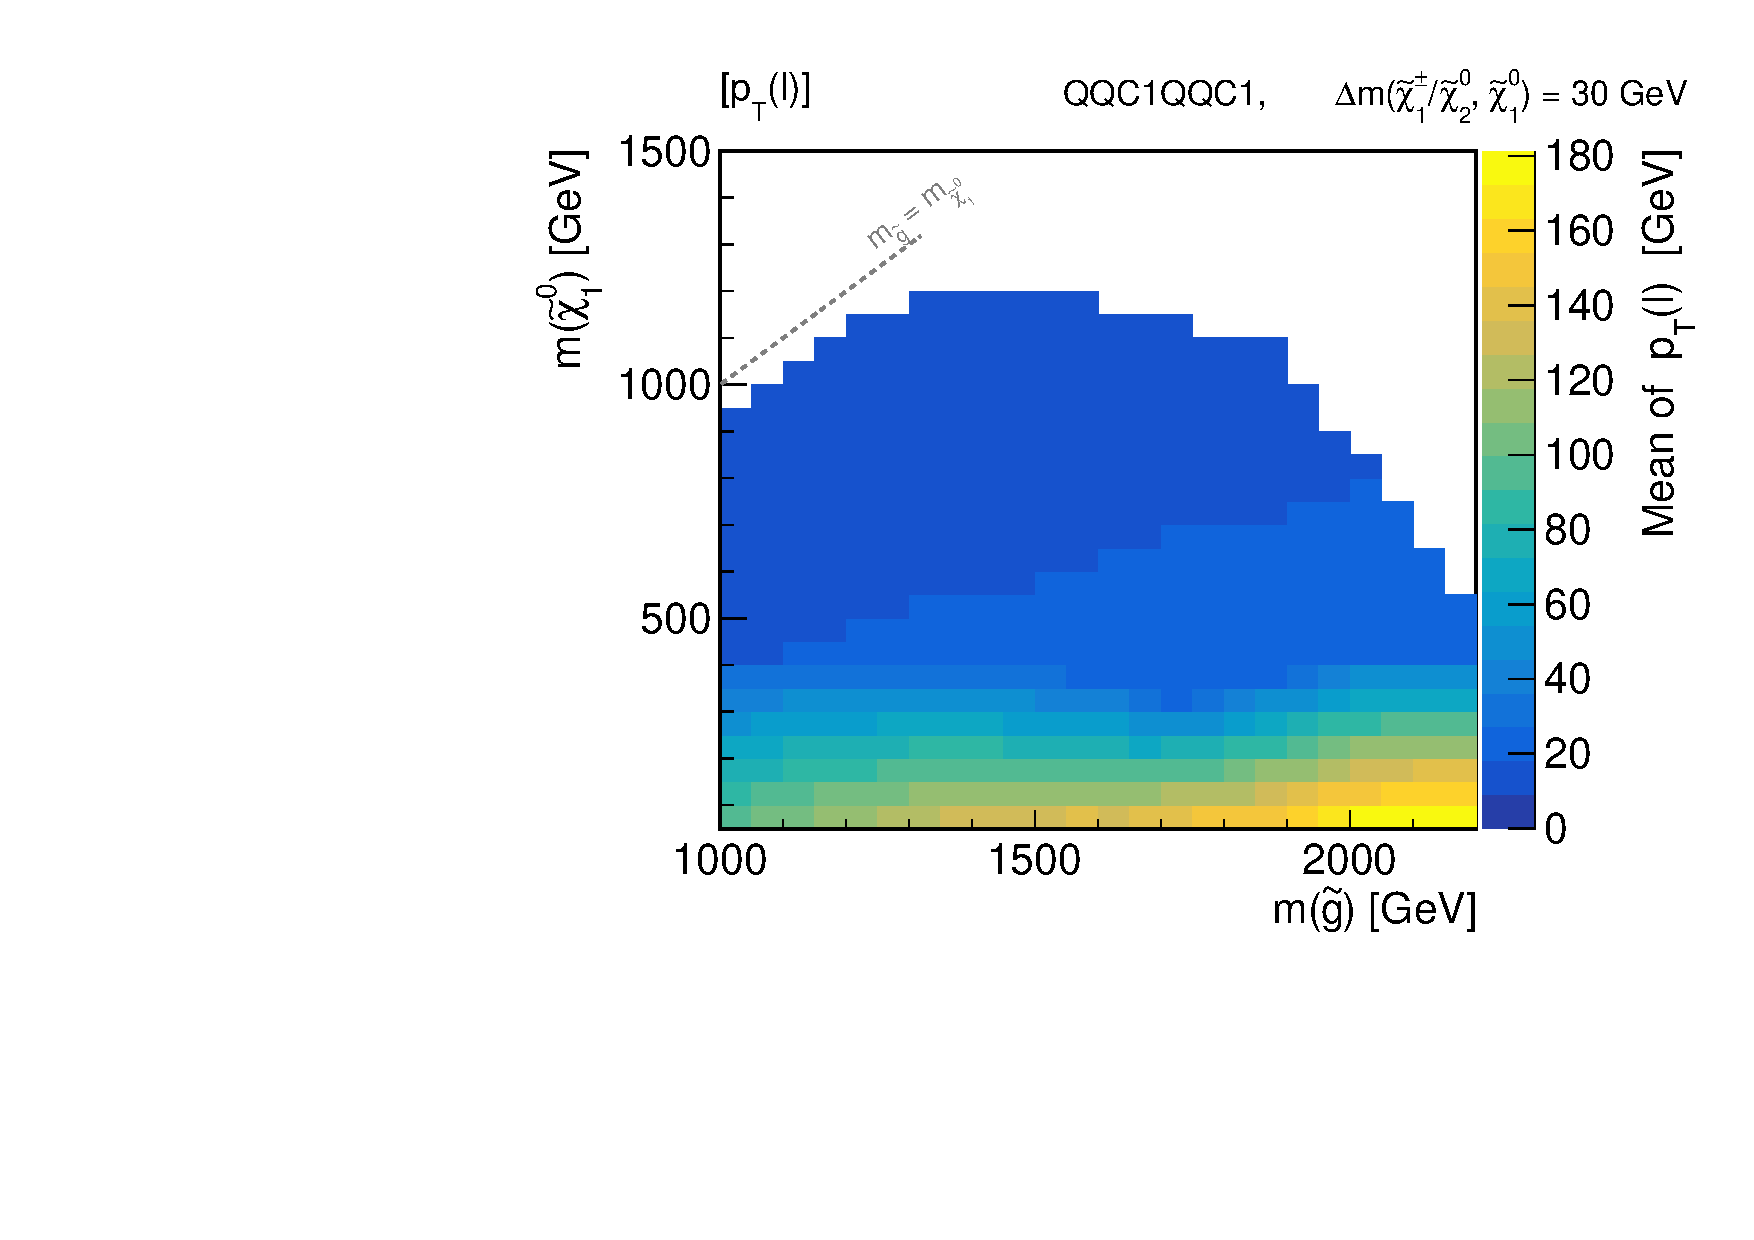
\includegraphics[width=0.45\textwidth]{figures/SRdefinition/kineMap/GG_symQQC1_dM30_lep1Pt.pdf}}
    \subfigure[]{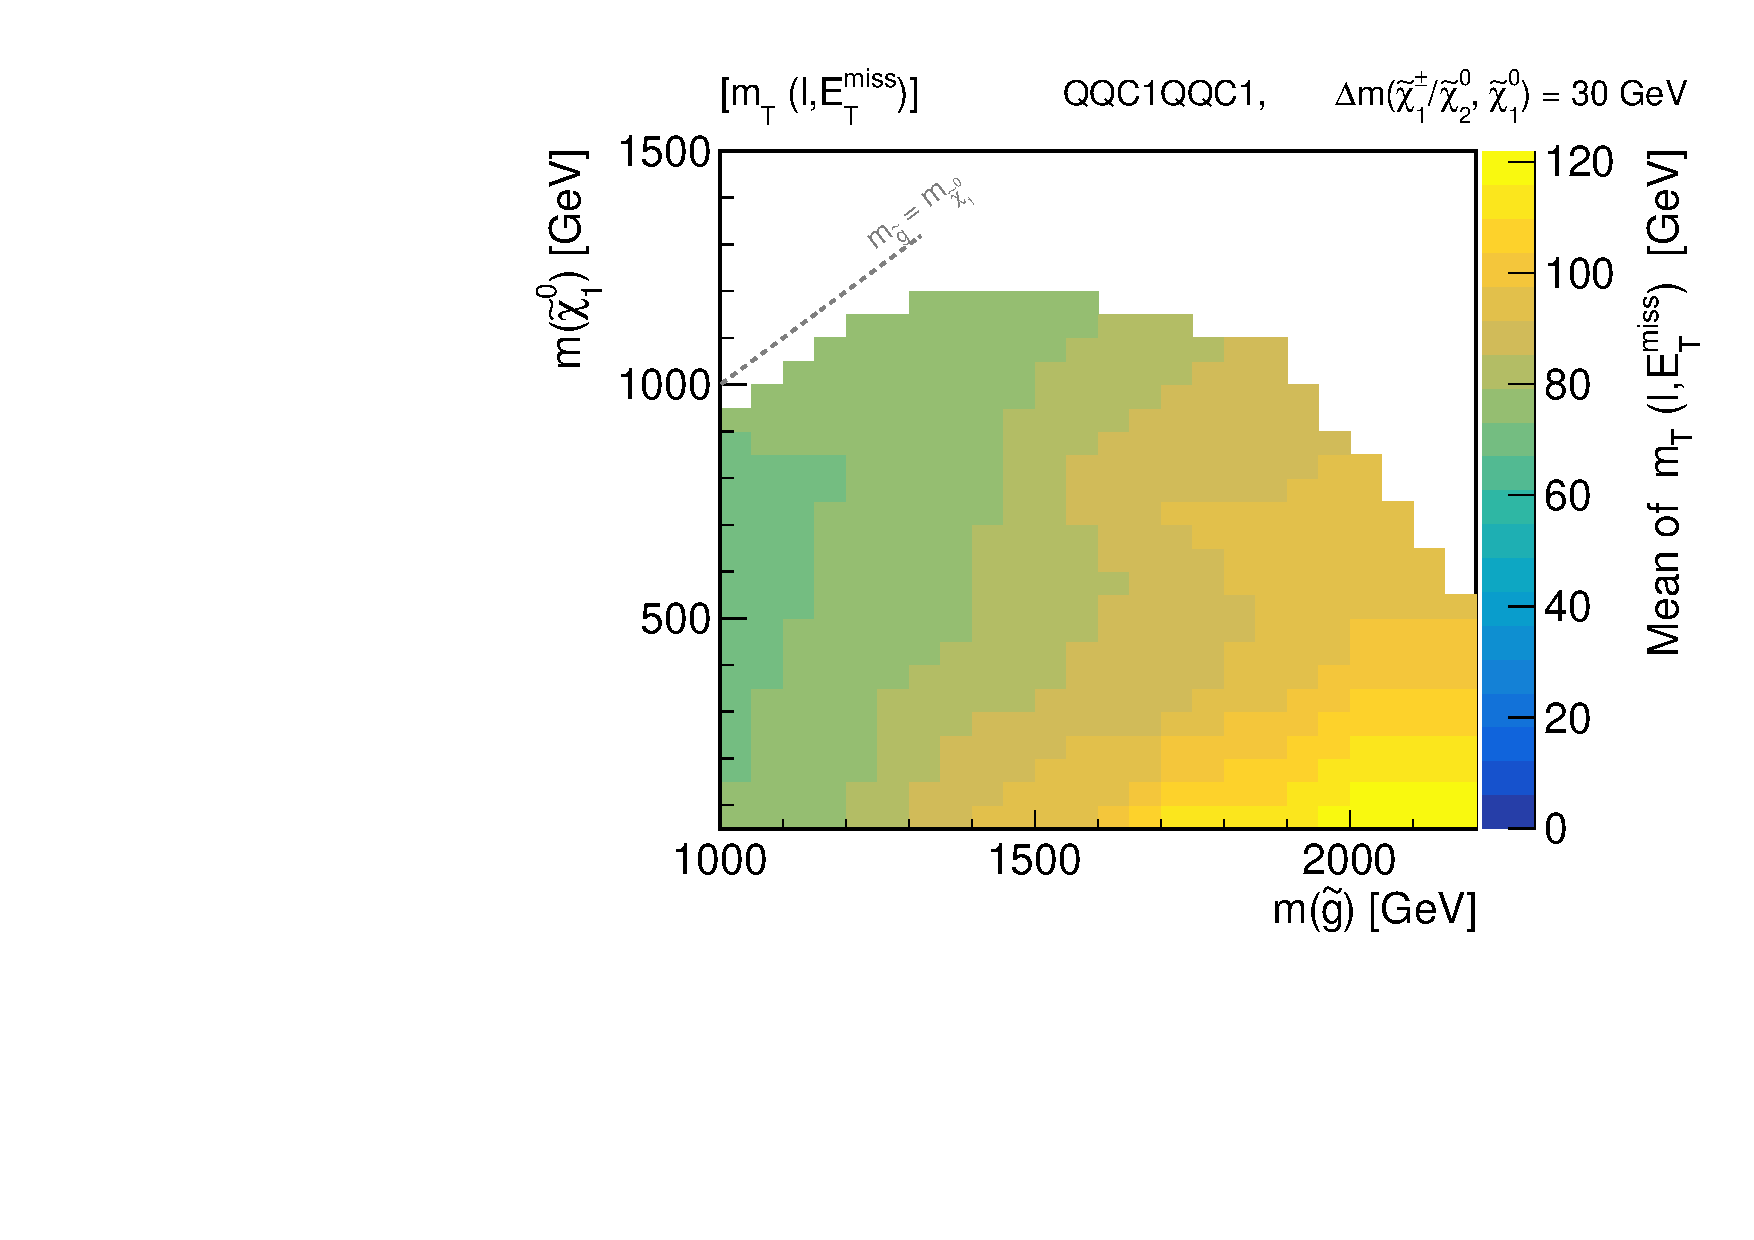
\includegraphics[width=0.45\textwidth]{figures/SRdefinition/kineMap/GG_symQQC1_dM30_mt.pdf}}
    \subfigure[]{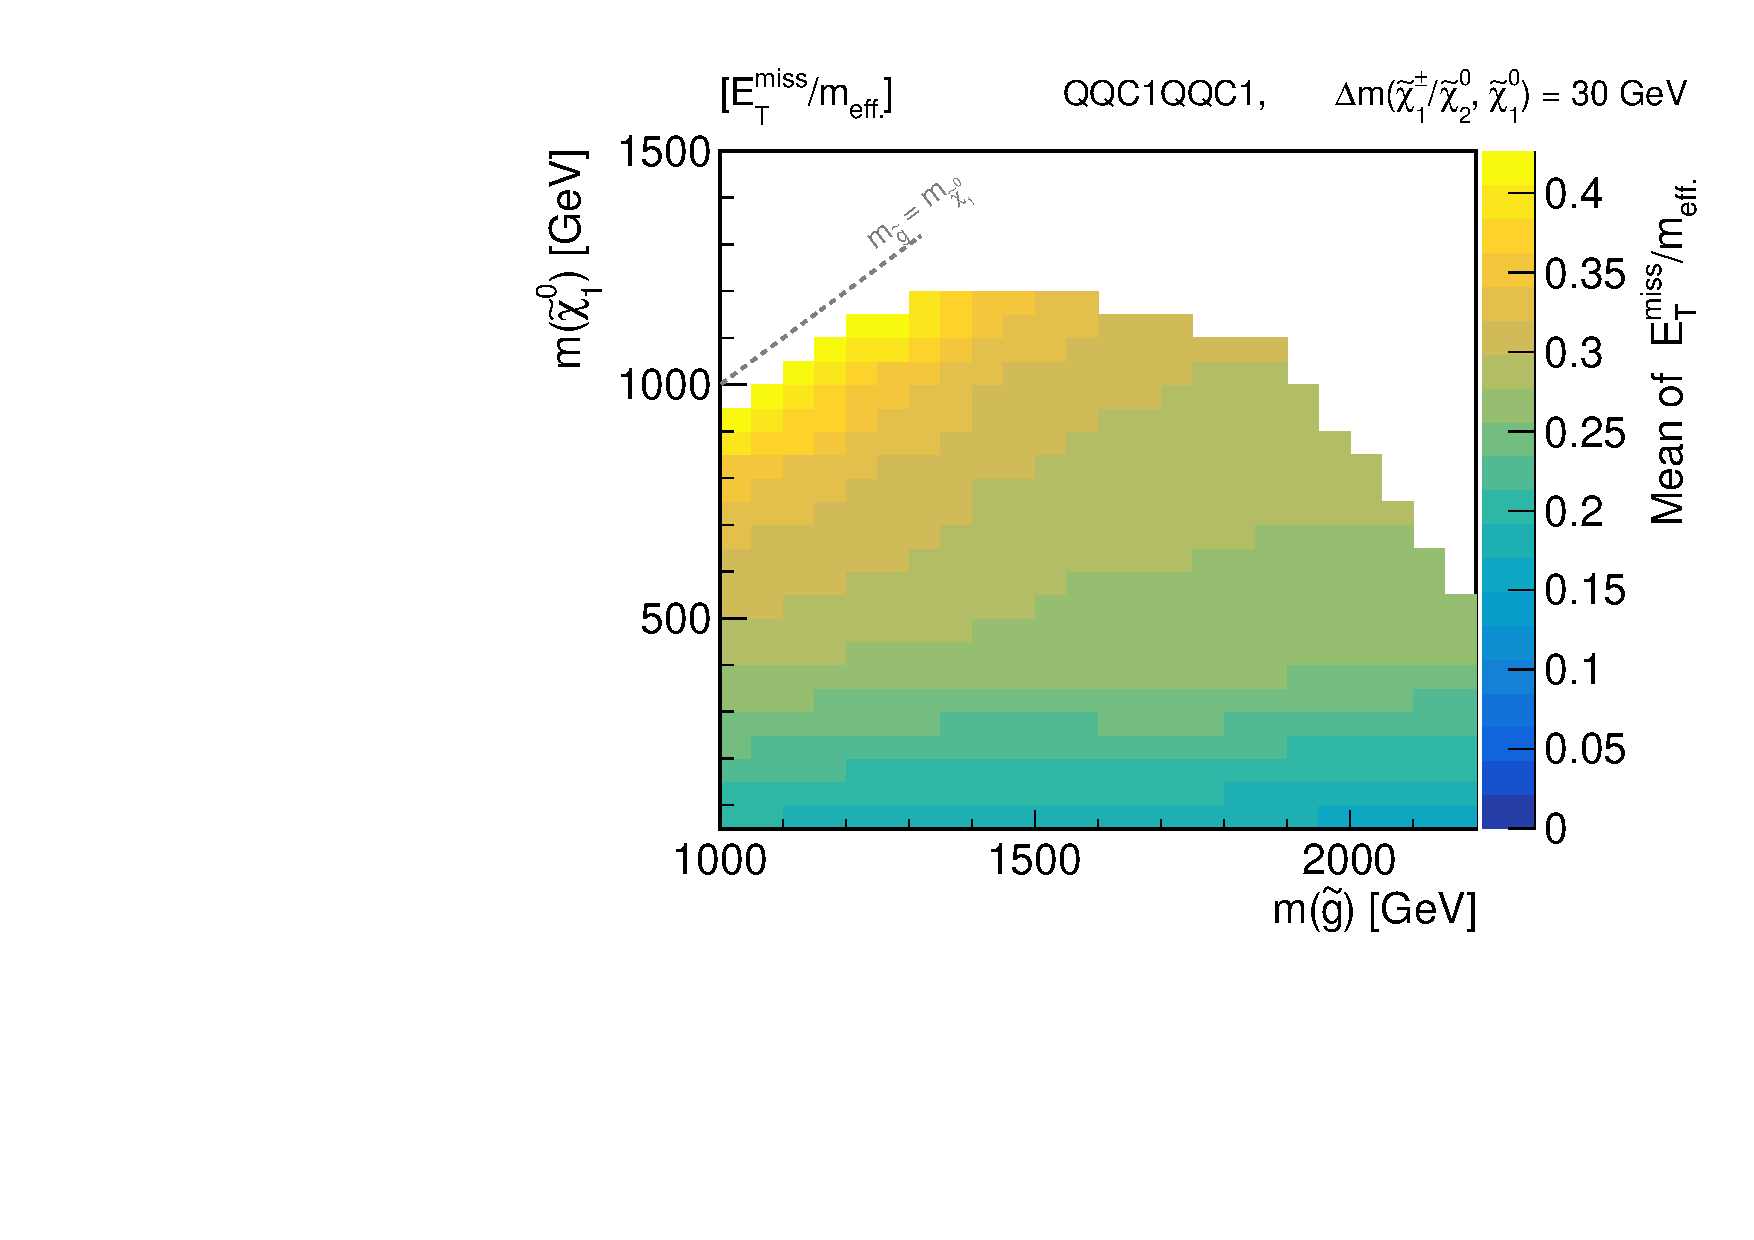
\includegraphics[width=0.45\textwidth]{figures/SRdefinition/kineMap/GG_symQQC1_dM30_metOverMeff.pdf}}
    \subfigure[]{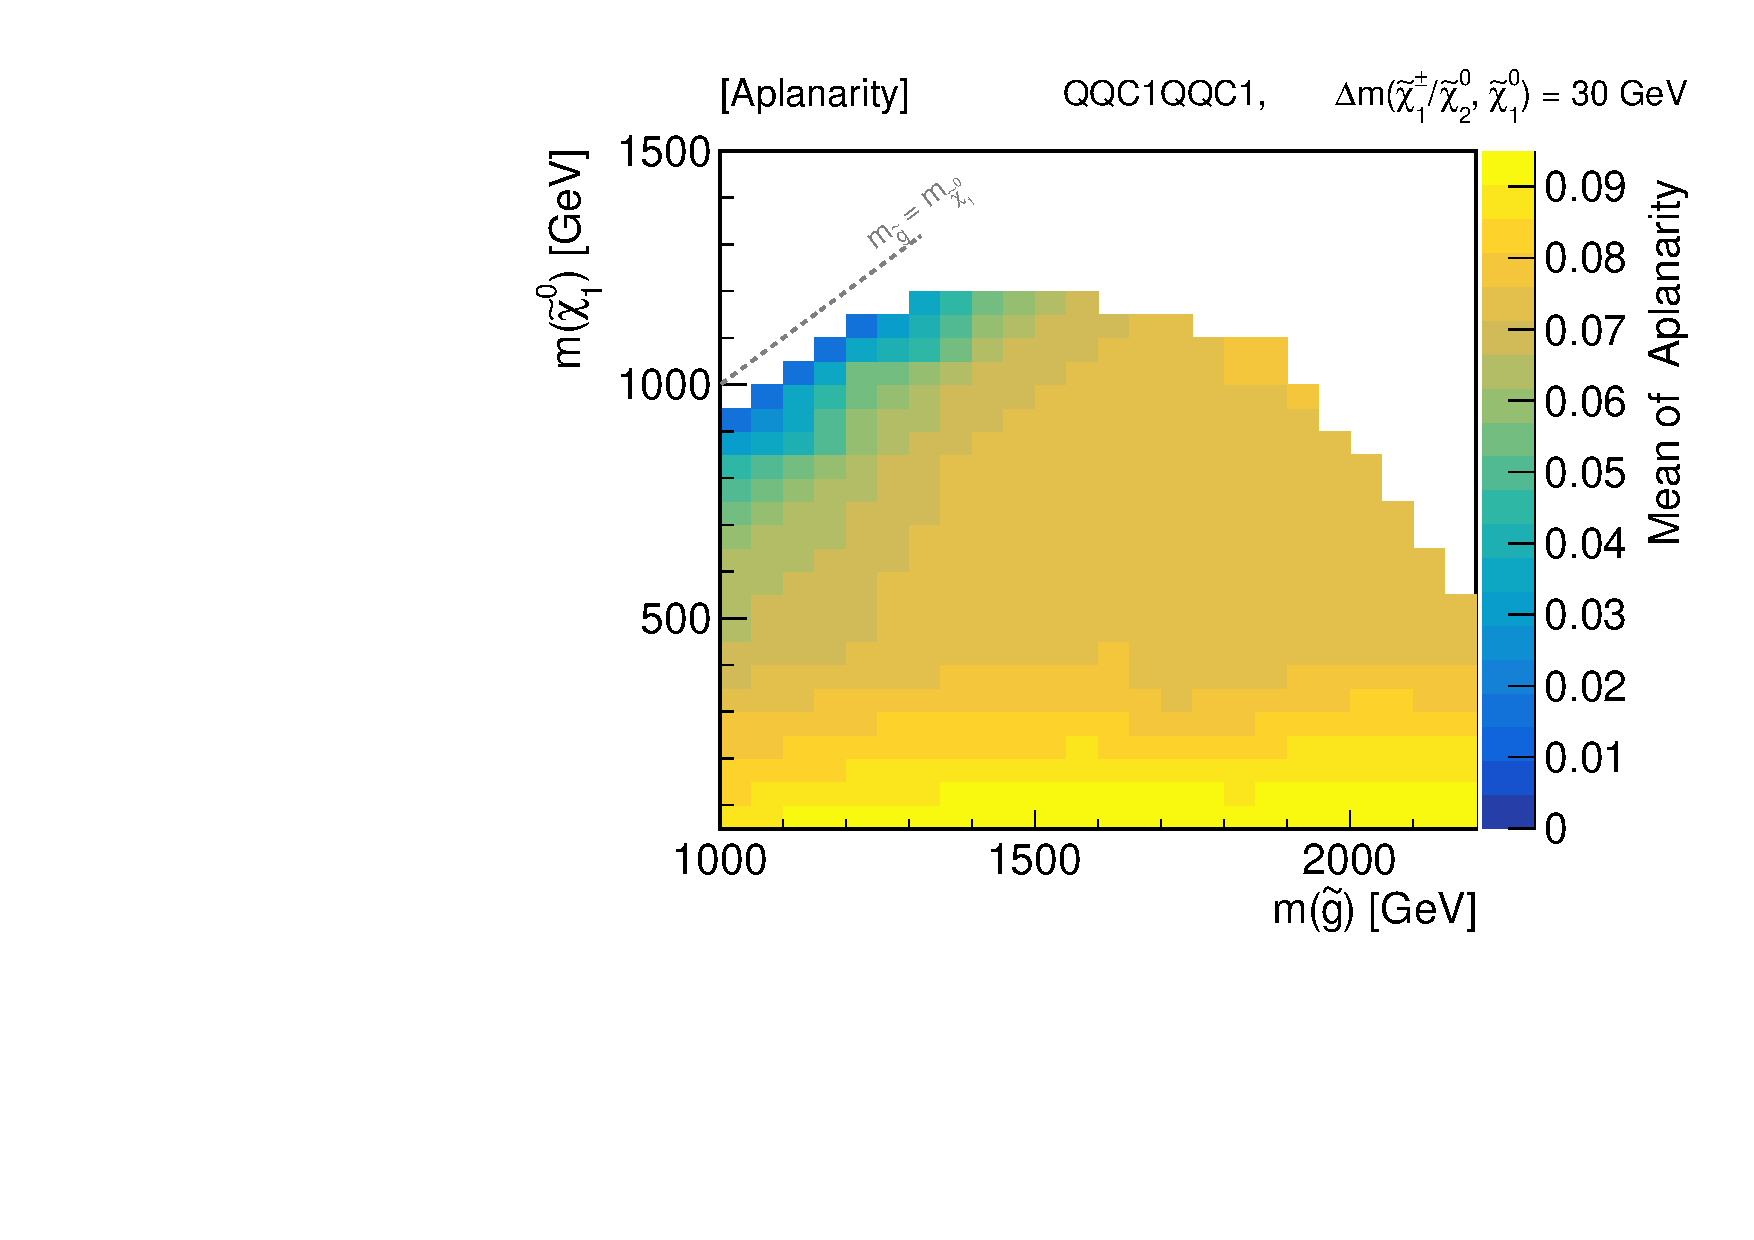
\includegraphics[width=0.45\textwidth]{figures/SRdefinition/kineMap/GG_symQQC1_dM30_LepAplanarity.pdf}}
    \caption{ Mean of (a) $\meffInc$ (b) $\met$ (c) $\lepPt$ (d) $\mt$ (e) $\metOverMeff$ (f) aplanarity, for the QQC1QQC1 \DMth grid, after the pre-selection. 
      \label{fig::SRdefinition::kineMap_QQC1QQC1_dM30} 
    }
\end{figure}


\begin{figure}[h]
  \centering
    \subfigure[]{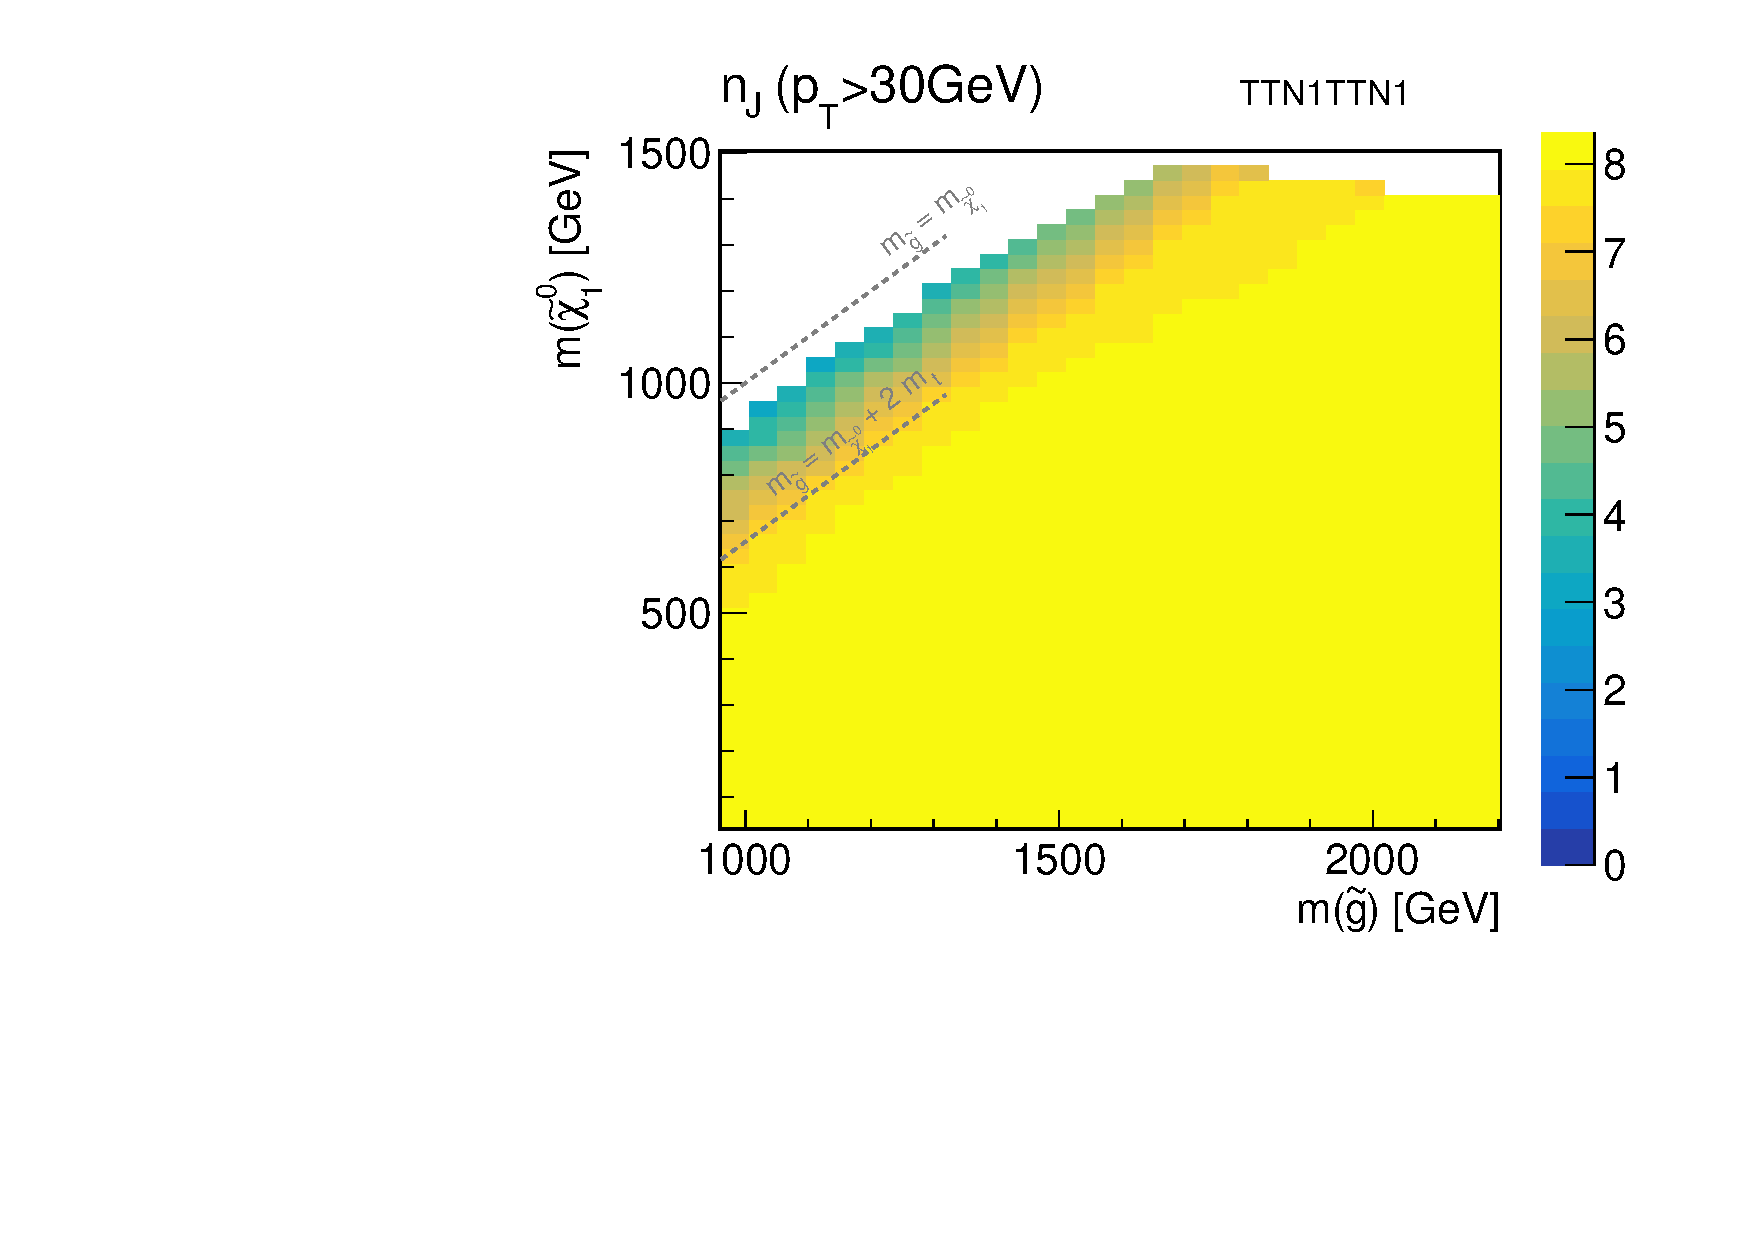
\includegraphics[width=0.32\textwidth]{figures/SRdefinition/kineMap/GG_symTTN1_x12_nJet30.pdf}}
    \subfigure[]{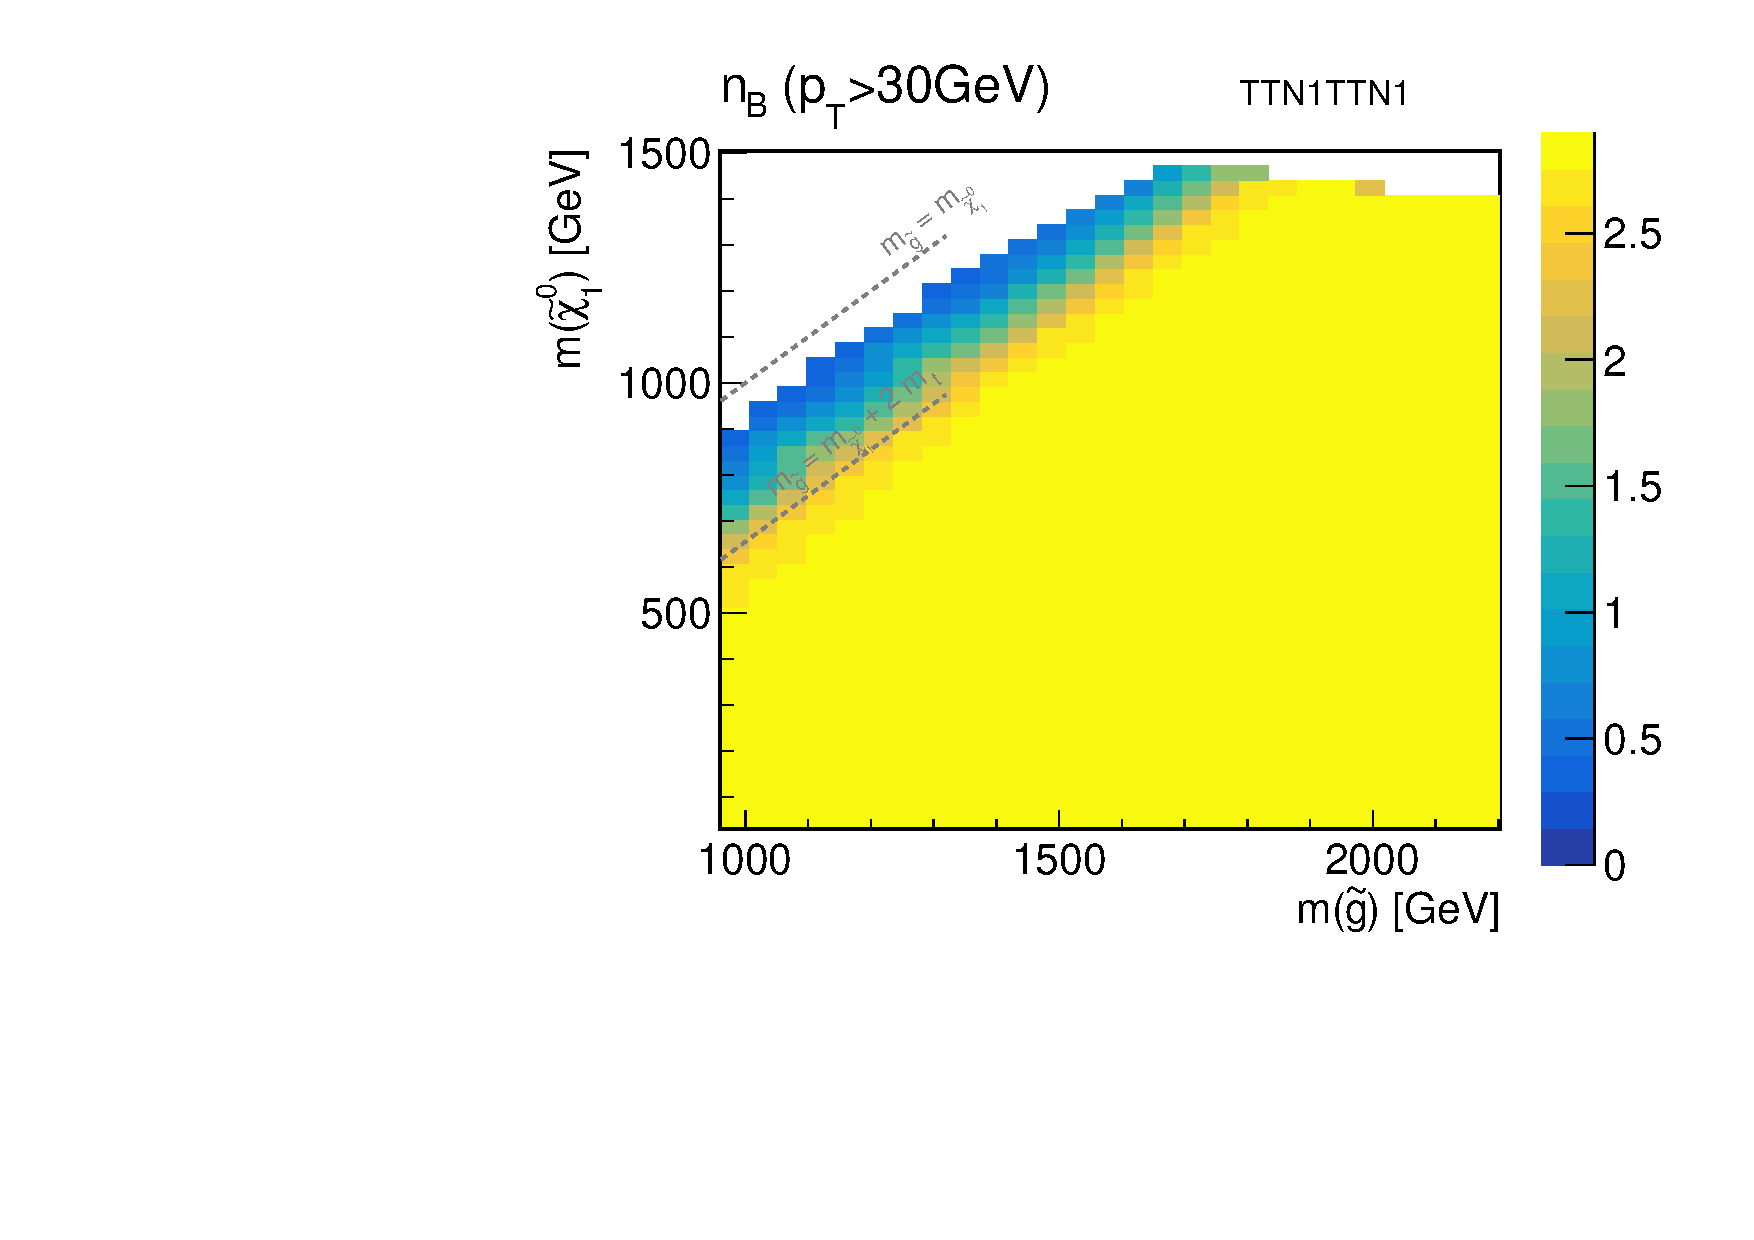
\includegraphics[width=0.32\textwidth]{figures/SRdefinition/kineMap/GG_symTTN1_x12_nBJet30.pdf}}
    \subfigure[]{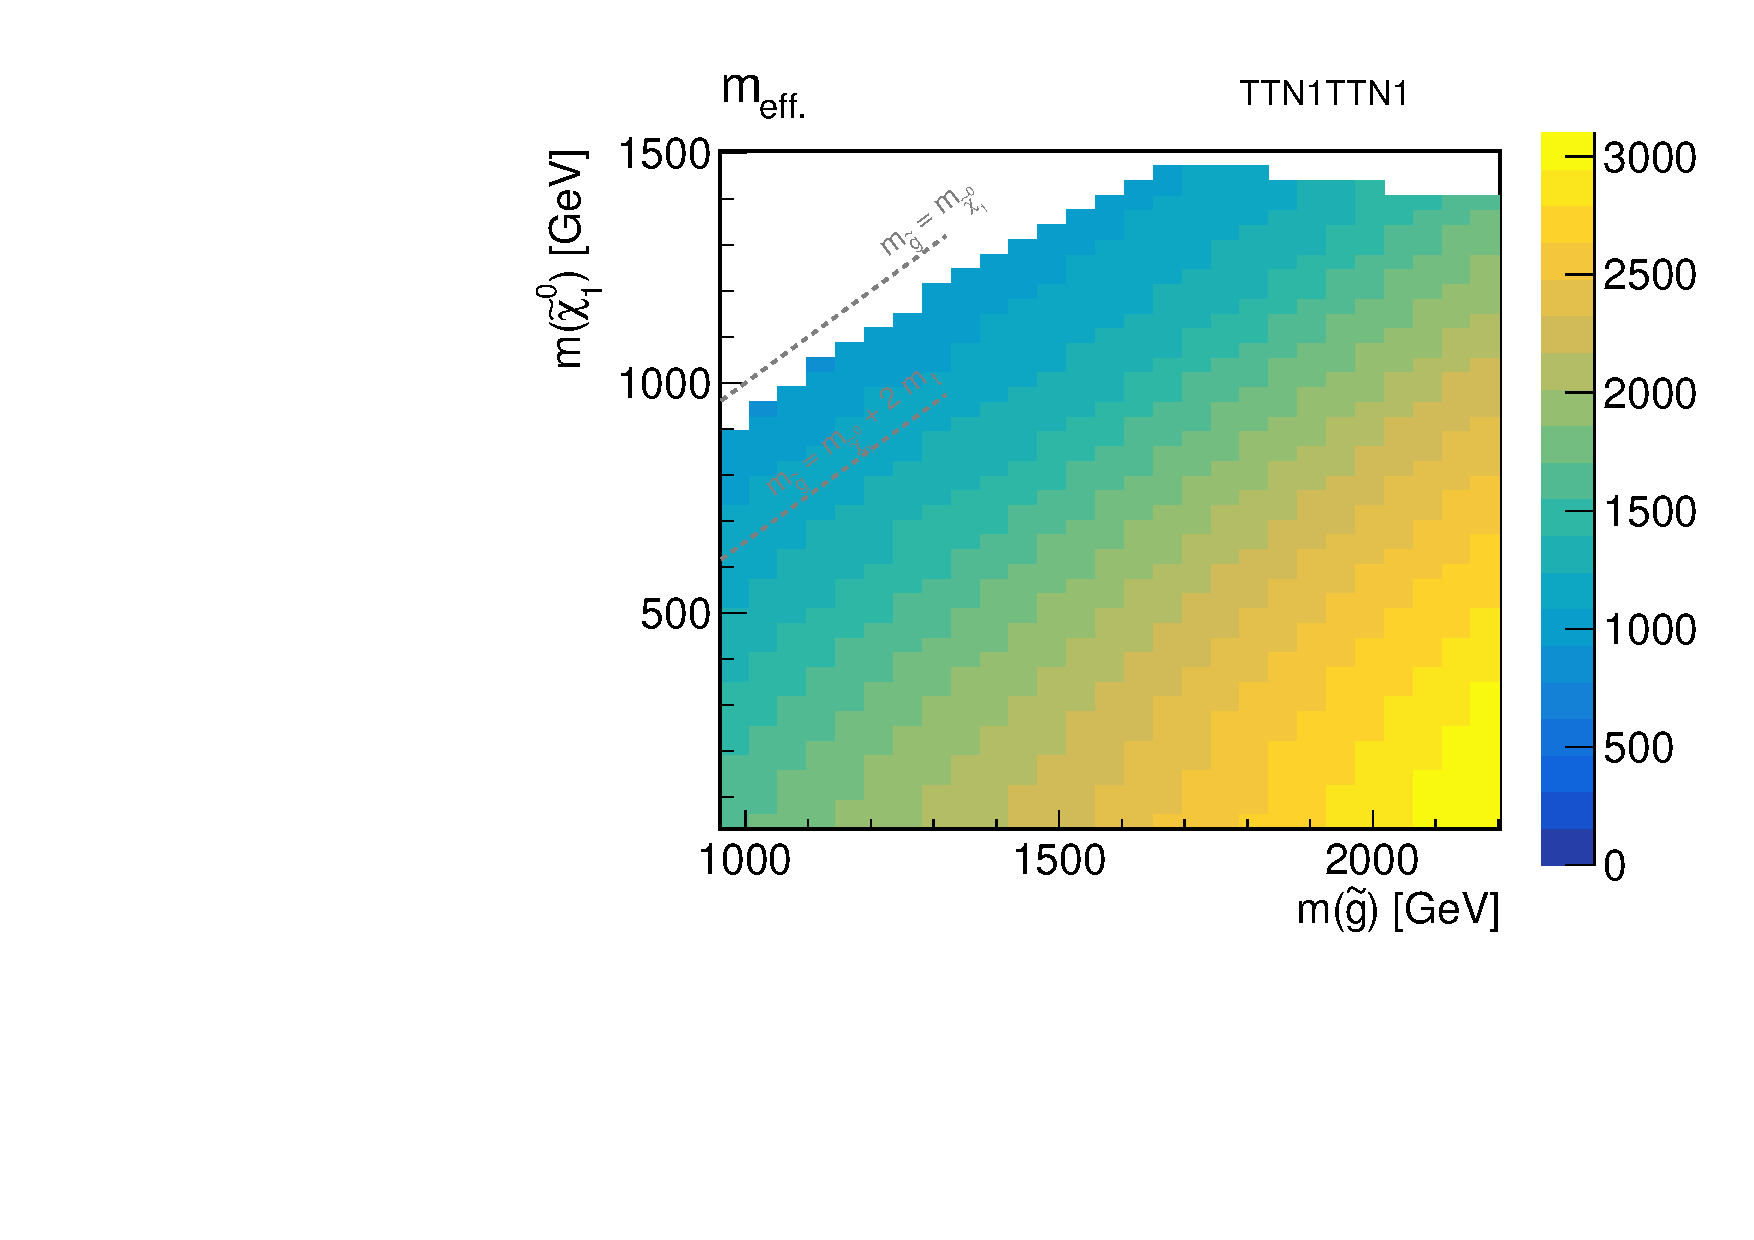
\includegraphics[width=0.32\textwidth]{figures/SRdefinition/kineMap/GG_symTTN1_x12_meff.pdf}}
    \subfigure[]{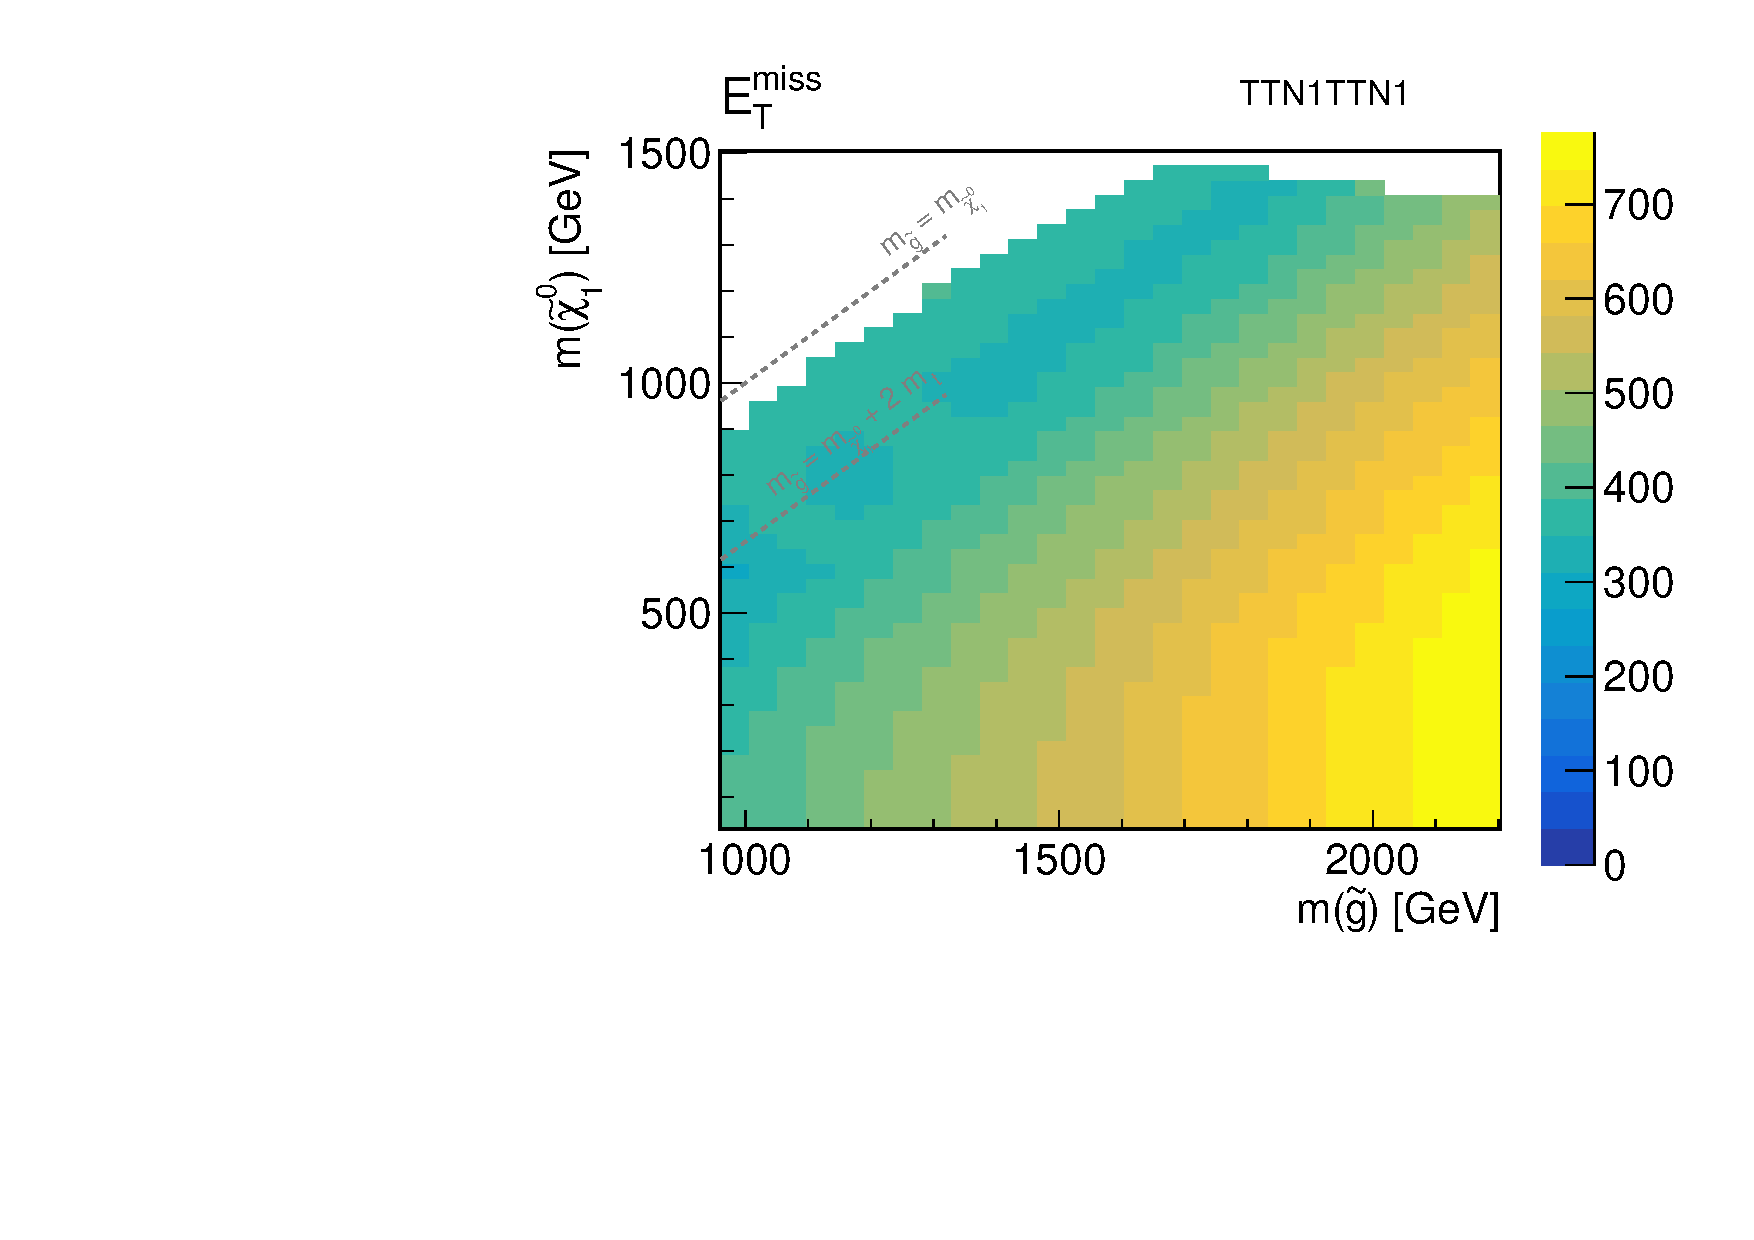
\includegraphics[width=0.32\textwidth]{figures/SRdefinition/kineMap/GG_symTTN1_x12_met.pdf}}
    \subfigure[]{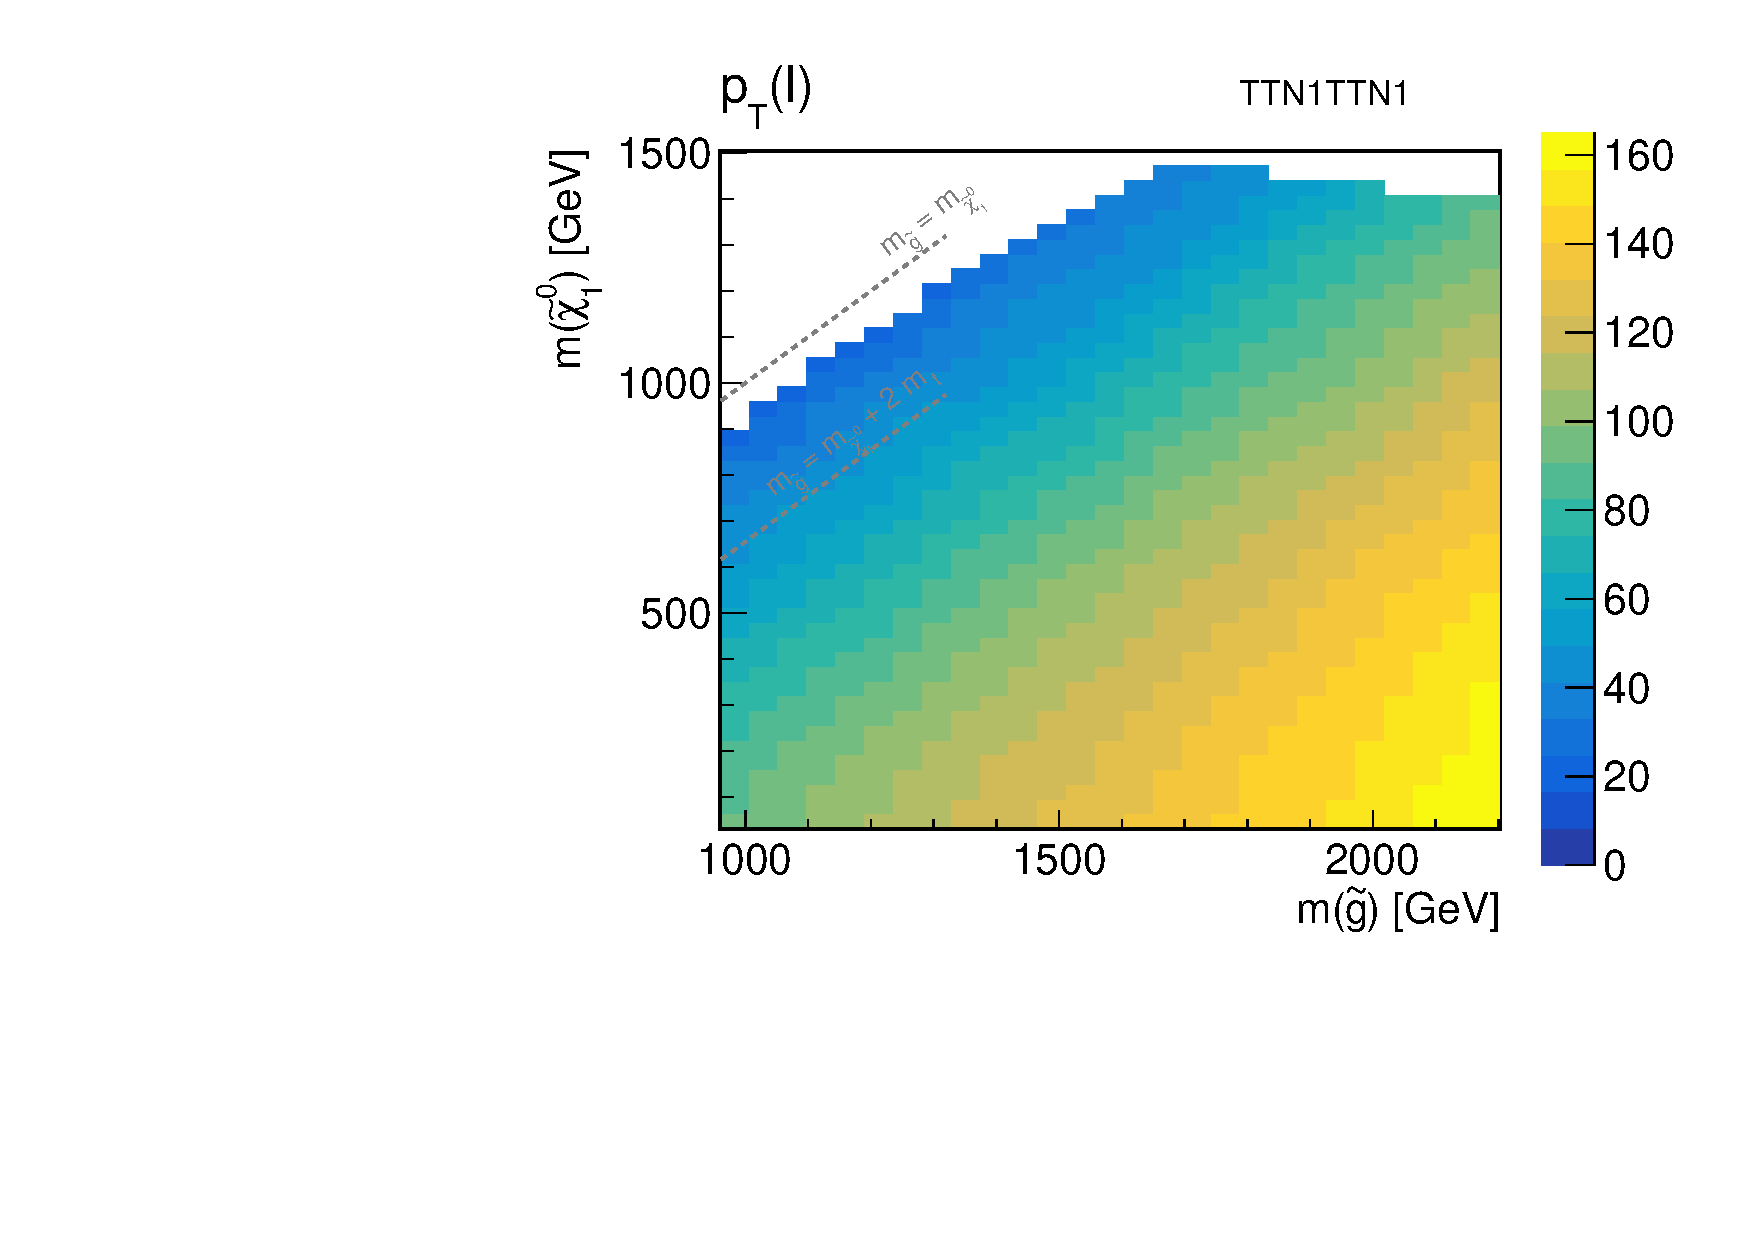
\includegraphics[width=0.32\textwidth]{figures/SRdefinition/kineMap/GG_symTTN1_x12_lep1Pt.pdf}}
    \subfigure[]{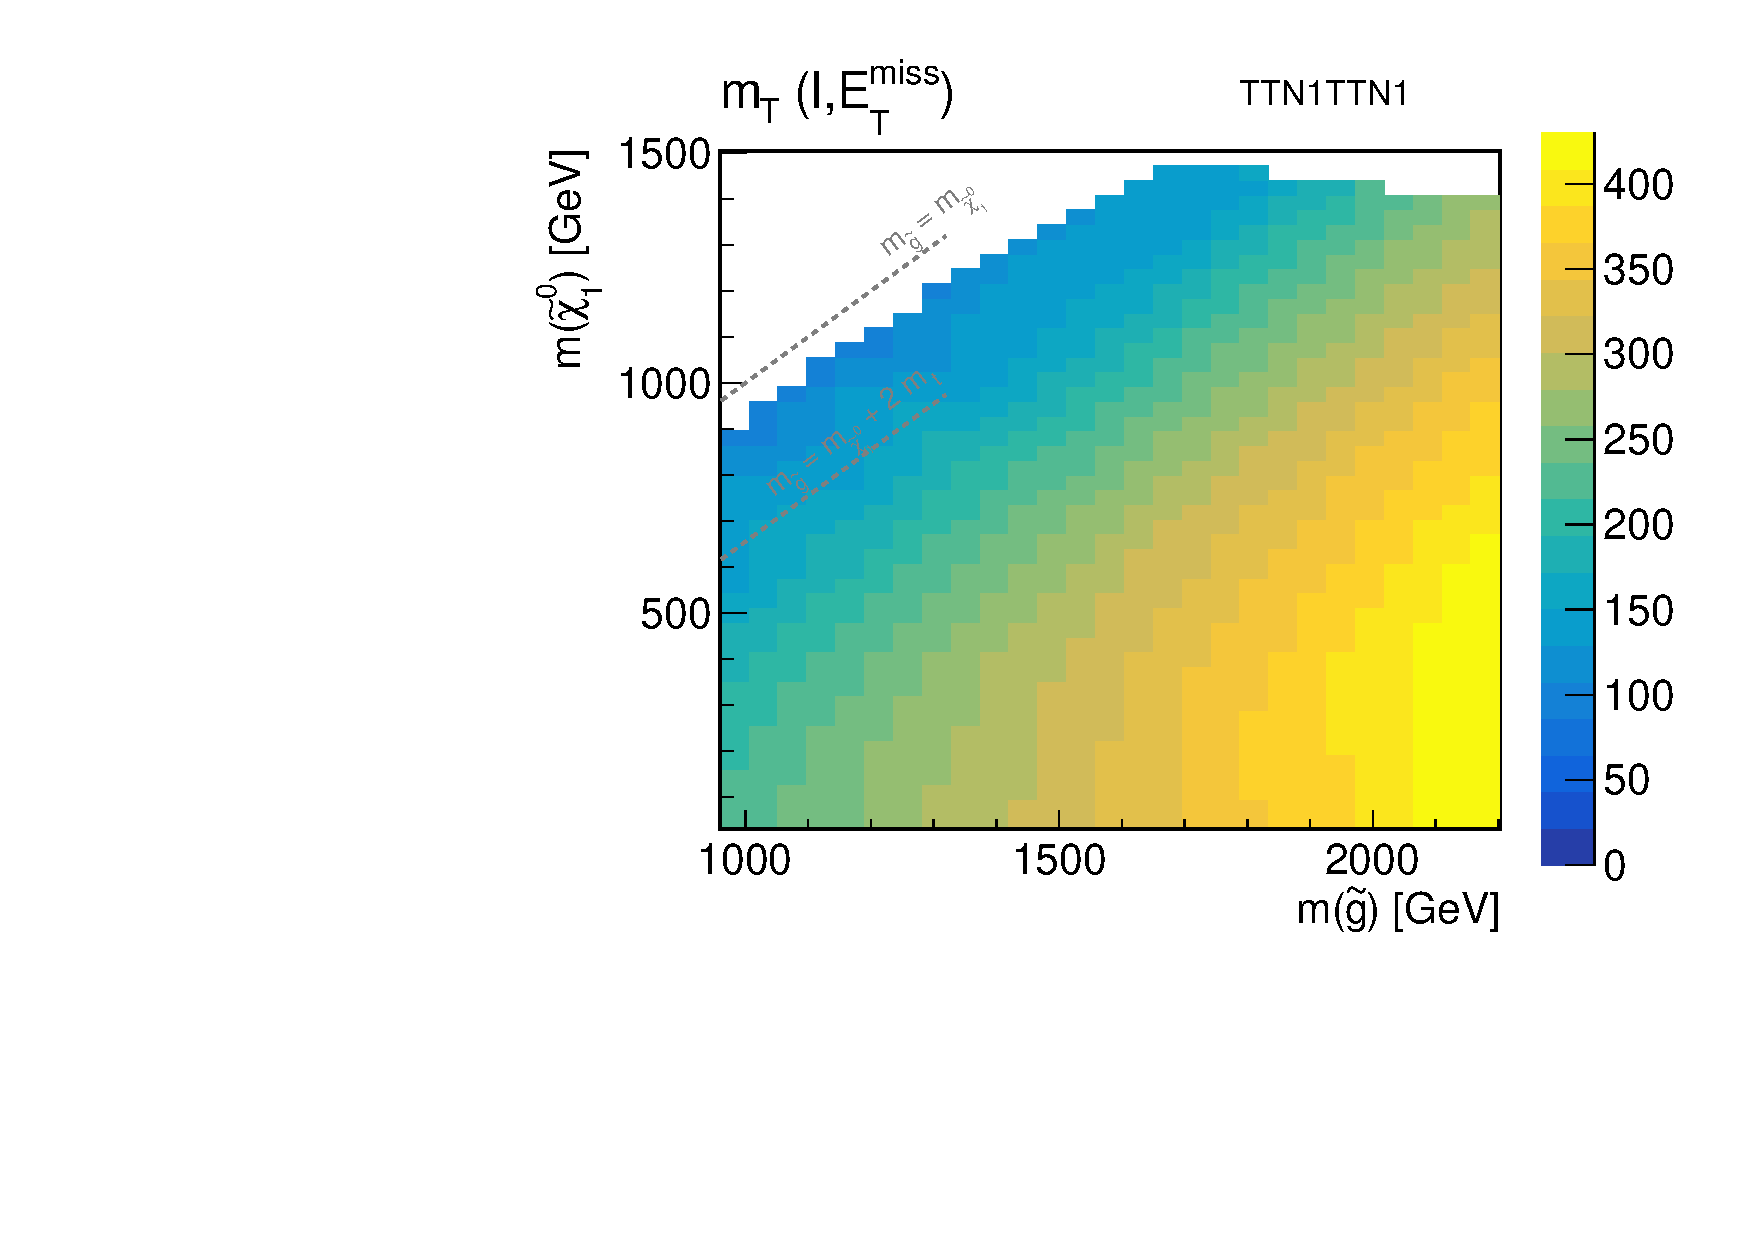
\includegraphics[width=0.32\textwidth]{figures/SRdefinition/kineMap/GG_symTTN1_x12_mt.pdf}}
    \subfigure[]{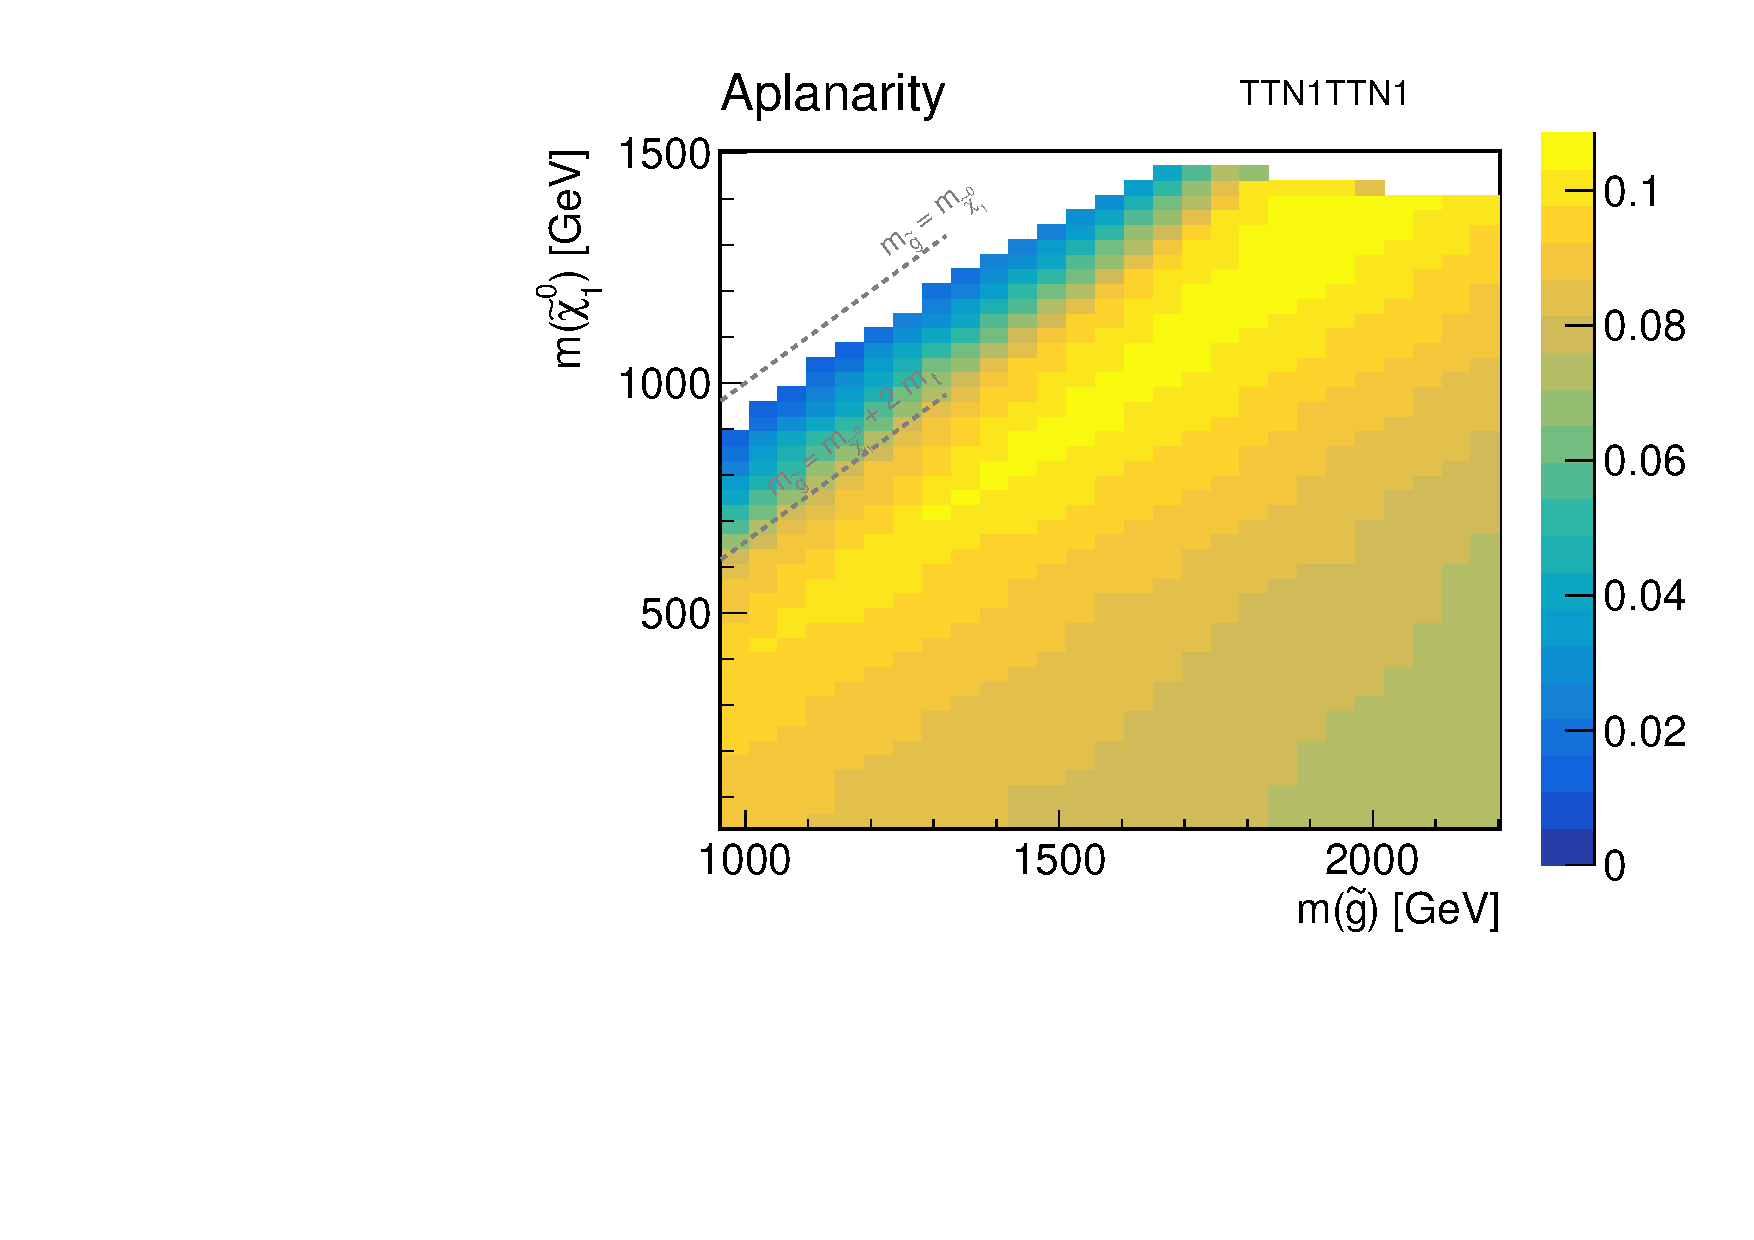
\includegraphics[width=0.32\textwidth]{figures/SRdefinition/kineMap/GG_symTTN1_x12_LepAplanarity.pdf}}
    \subfigure[]{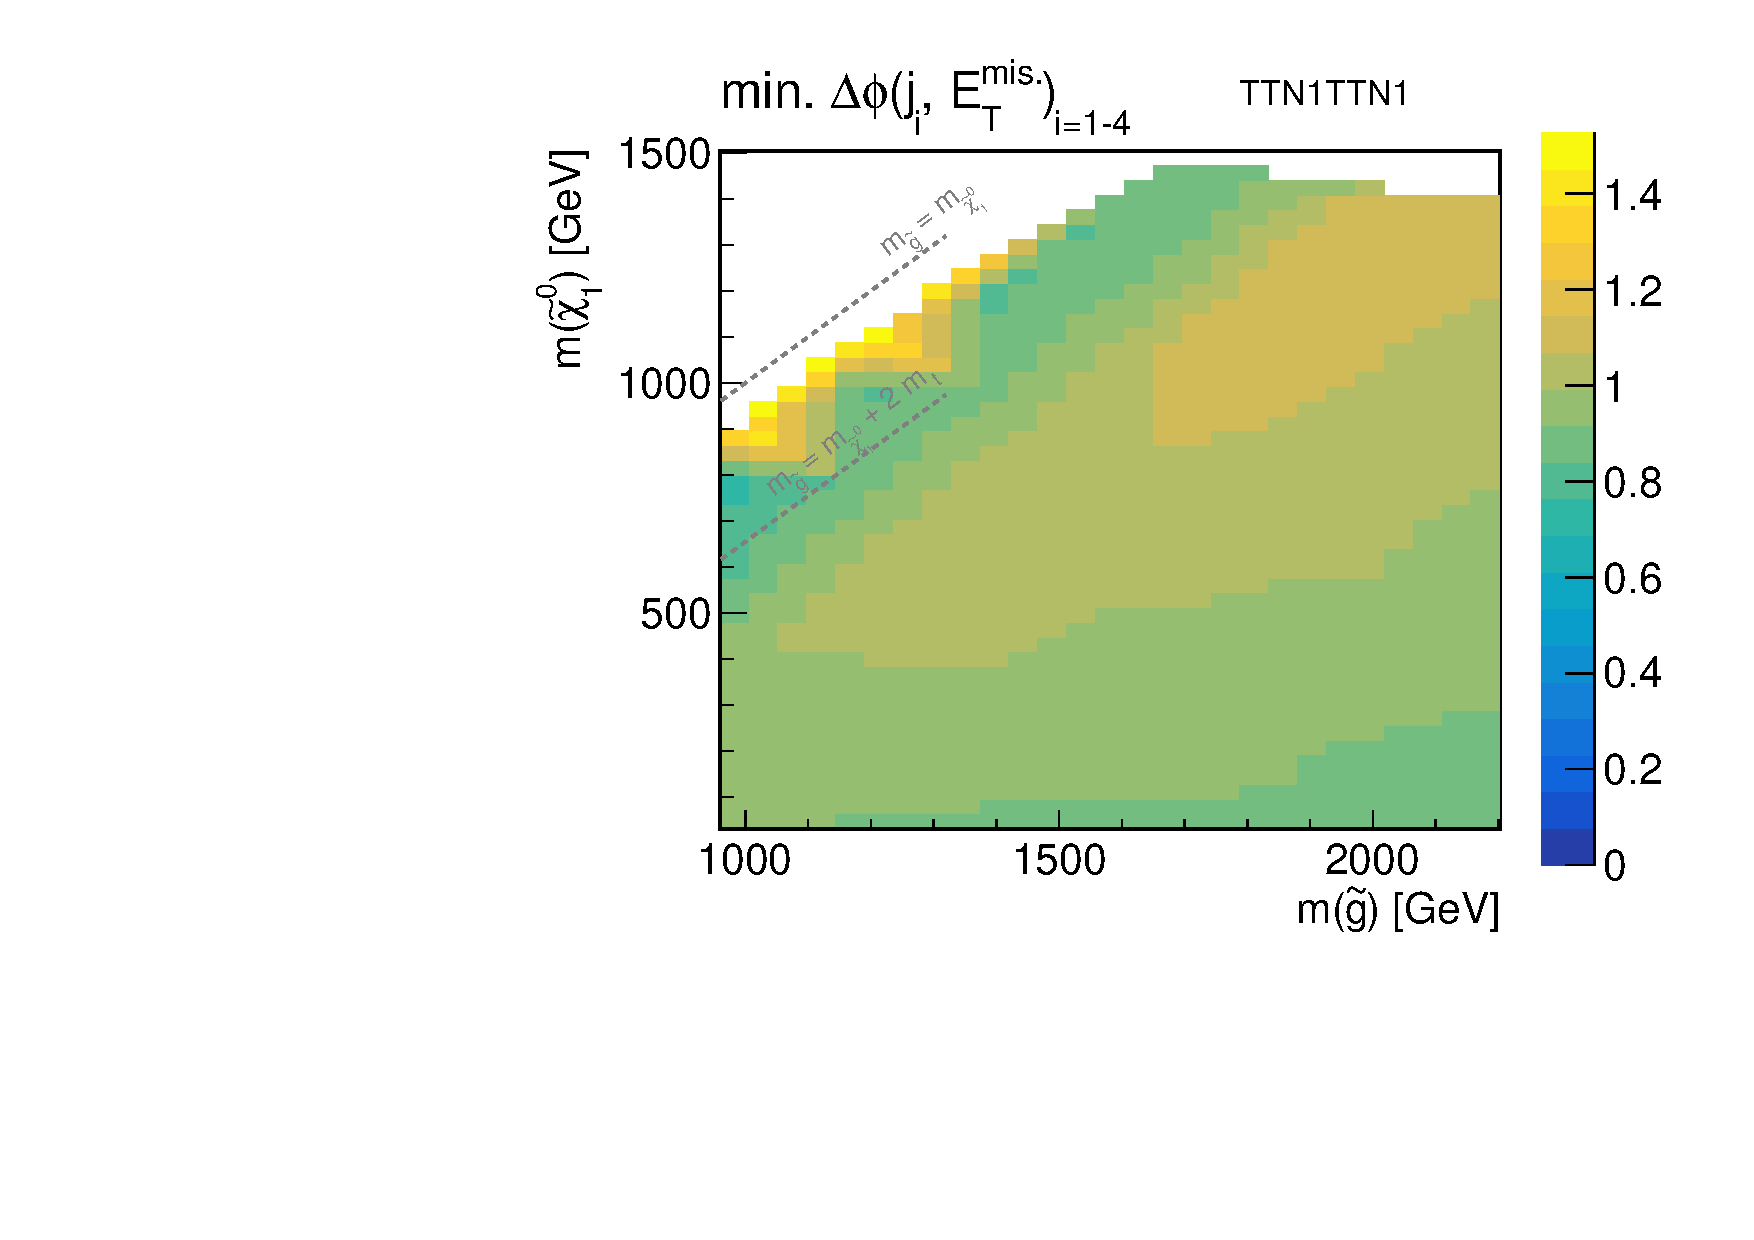
\includegraphics[width=0.32\textwidth]{figures/SRdefinition/kineMap/GG_symTTN1_x12_min_dPhi_4j.pdf}}
    \subfigure[]{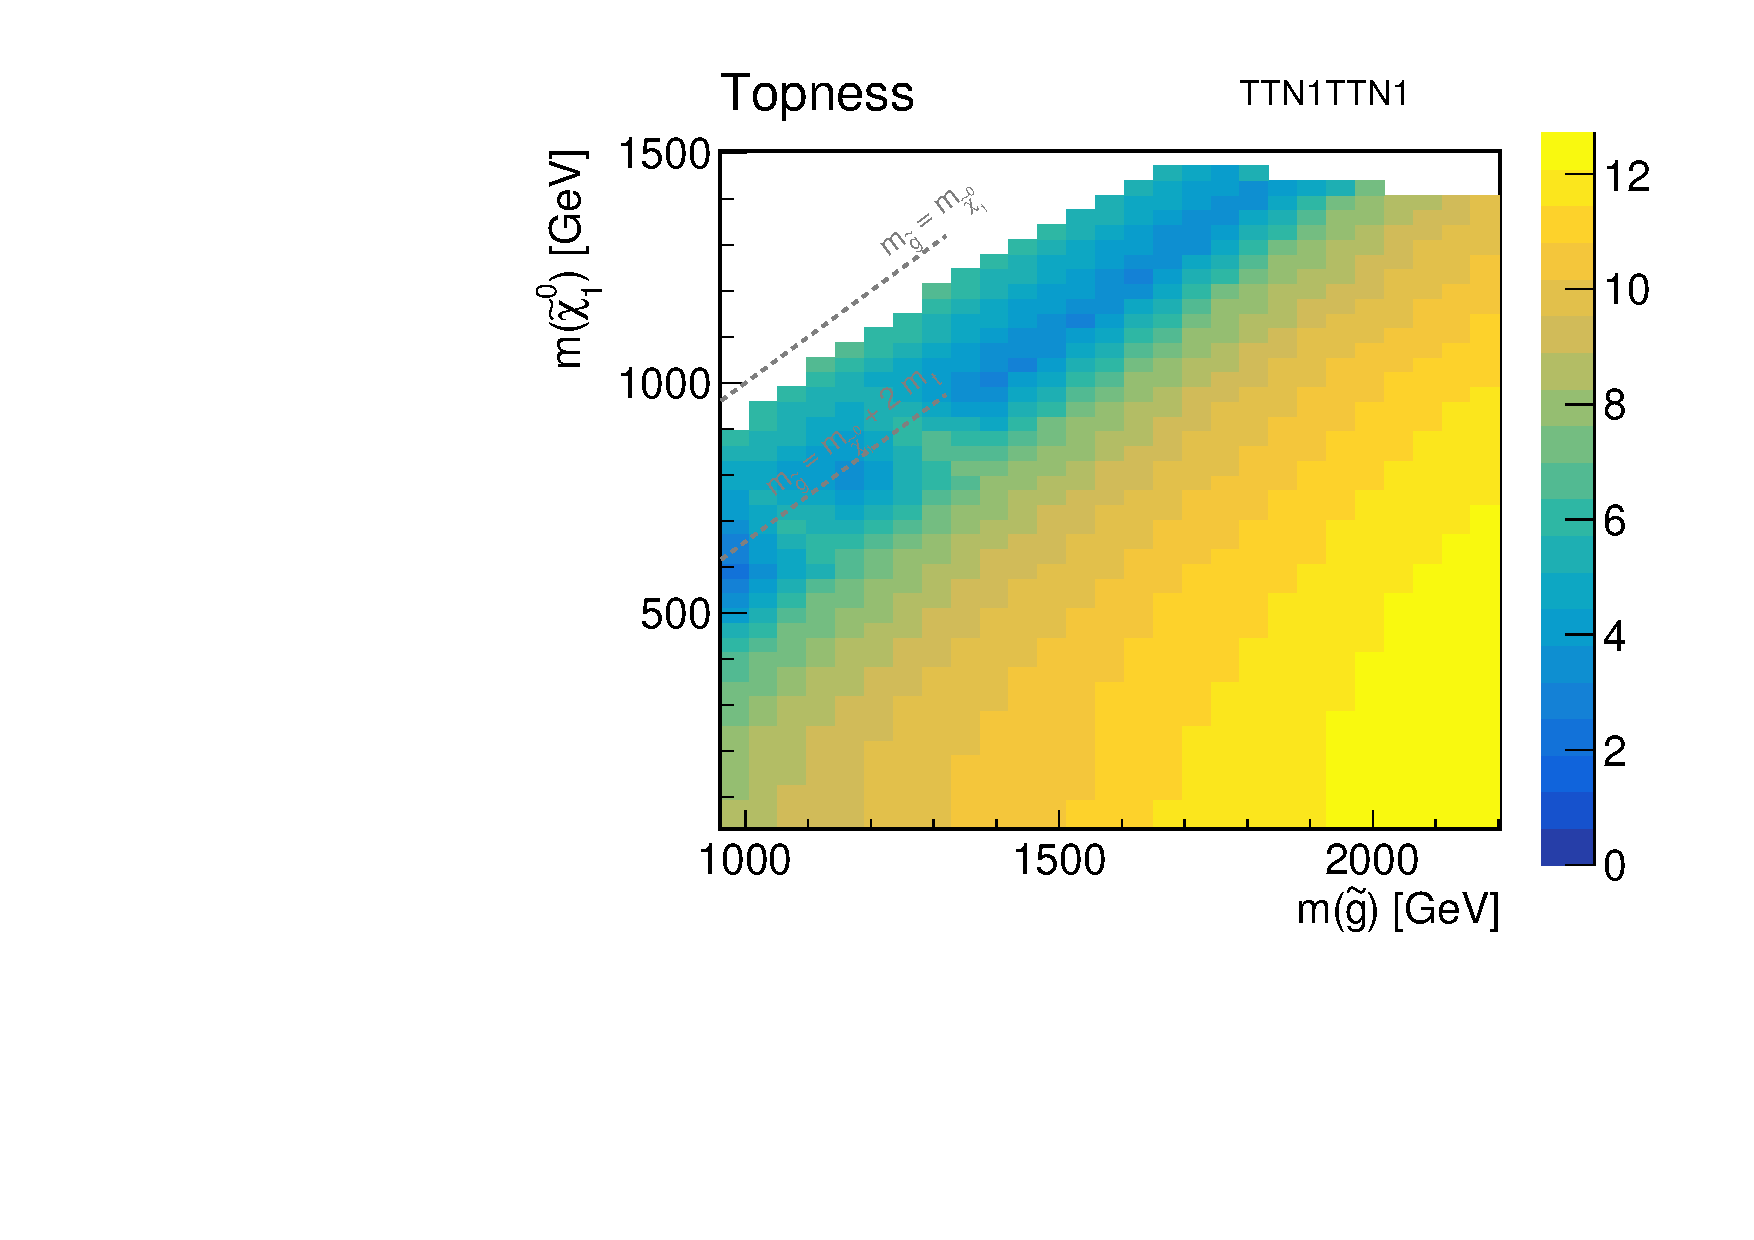
\includegraphics[width=0.32\textwidth]{figures/SRdefinition/kineMap/GG_symTTN1_x12_topNess.pdf}}
    \caption{ Mean of (a) jet-multiplicity ($p_T>30\gev$) (b) bjet-multiplicity ($p_T>30\gev$) (c) $\meffInc$ (d) $\met$ (e) $\lepPt$ (f) $\mt$ (g) aplanarity (h) $\mindPhiFourJet$ (i) topness, for the TTN1TTN1 \dire grid, after the pre-selection. 
      \label{fig::SRdefinition::kineMap_TTN1TTN1} 
    }
\end{figure}
 

